\documentclass[13pt,a4paper]{article}
\usepackage[spanish,es-nodecimaldot]{babel}	% Utilizar español
\usepackage[utf8]{inputenc}					% Caracteres UTF-8
\usepackage{graphicx}						% Imagenes
\usepackage[hidelinks]{hyperref}			% Poner enlaces sin marcarlos en rojo
\usepackage{fancyhdr}						% Modificar encabezados y pies de pagina
\usepackage{float}							% Insertar figuras
\usepackage[textwidth=390pt]{geometry}		% Anchura de la pagina
\usepackage[nottoc]{tocbibind}				% Referencias (no incluir num pagina indice en Indice)
\usepackage{enumitem}						% Permitir enumerate con distintos simbolos
\usepackage[T1]{fontenc}					% Usar textsc en sections
\usepackage{amsmath}						% Símbolos matemáticos
\usepackage[ruled,vlined]{algorithm2e}      % Pseudocódigo
\usepackage{xcolor}
\usepackage{listings}
\usepackage{dsfont}
\usepackage{subfigure}

% Comando para poner el nombre de la asignatura
\newcommand{\asignatura}{Introducción a la Ciencia de Datos}
\newcommand{\autor}{Ignacio Vellido Expósito}
\newcommand{\titulo}{Trabajo teórico/práctico}
\newcommand{\subtitulo}{Análisis de datos, Regresión y Clasificación}

% Configuracion de encabezados y pies de pagina
\pagestyle{fancy}
\lhead{\autor{}}
\rhead{\asignatura{}}
\lfoot{Máster Ciencia de Datos e Ingeniería de Computadores}
\cfoot{}
\rfoot{\thepage}
\renewcommand{\headrulewidth}{0.4pt}		% Linea cabeza de pagina
\renewcommand{\footrulewidth}{0.4pt}		% Linea pie de pagina

% ==============================================================================
% ==============================================================================

\begin{document}
    \pagenumbering{gobble}
    % ==============================================================================
% Pagina de titulo
\begin{titlepage}
    \begin{minipage}{\textwidth}
        \centering

        
\includegraphics[scale=0.5]{img/ugr.png}\\

        \textsc{\Large \asignatura{}\\[0.2cm]}
        \textsc{MÁSTER CIENCIA DE DATOS E INGENIERÍA DE COMPUTADORES}\\[1cm]

        \noindent\rule[-1ex]{\textwidth}{1pt}\\[1.5ex]
        \textsc{{\Huge \titulo\\[0.5ex]}}
        \textsc{{\Large \subtitulo\\}}
        \noindent\rule[-1ex]{\textwidth}{2pt}\\[2.5ex]

        \end{minipage}

        \vspace{0.3cm}

        \begin{minipage}{\textwidth}

        \centering

        \textbf{Autor}\\ {\autor{} \\ ignaciove@correo.ugr.es}\\[1.5ex]
        \vspace{0.4cm}

        
\includegraphics[scale=0.3]{img/etsiit.jpeg}
        
\includegraphics[scale=0.6]{img/master.png}

        \vspace{0.7cm}
        \textsc{Escuela Técnica Superior de Ingenierías Informática y de Telecomunicación}\\
        \vspace{1cm}
        \textsc{Curso 2020-2021}
    \end{minipage}
\end{titlepage}
% ==============================================================================
    
    \pagenumbering{arabic}
    \tableofcontents
    \thispagestyle{empty}				% No usar estilo en la pagina de indice

    \newpage

    % ==============================================================================

    % \section{Introducción} \newpage
    % \input{secciones/eda} \newpage
    % \section{Técnicas de Regresión}

Recordamos que la descripción de los datos se encuentra en el apartado 1.1.

\vspace{\baselineskip}

Como se comentó en las conclusiones del análisis estadístico:

``Se nos pide elegir 5 regresores para la regresión y contamos exactamente con ese número, por lo que no podemos descartar ninguna variable. Aún así, hemos visto que tenemos algunas variables más interesantes que otras. Variables correladas con la salida nos aumentan las posibilidades de obtener un buen regresor, pero debemos evitar usar variables correladas entre sí para evitar la multicolinealidad, y aumentar la interpretabilidad del modelo, pero la potencia en sí de este no cambia.''

\vspace{\baselineskip}

Primeramente, mostramos la relación de cada variable respecto a la salida:

\begin{figure}[H]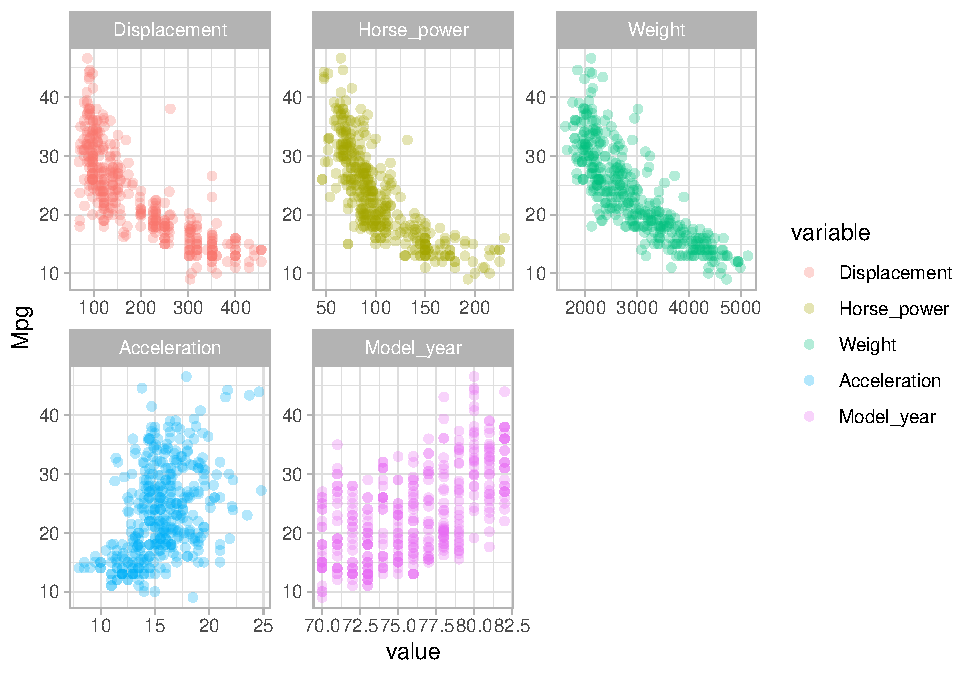
\includegraphics[width=.9\linewidth]{img/Regresion_files/figure-latex/unnamed-chunk-2-1} \caption{}\end{figure}

Como dijimos, se aprecia alta correlación entre Displacement, Horse\_power, Weight respecto de la salida, probablemente de forma logarítmica.

Las matrices de correlación nos confirmaban esta idea (con coeficientes de Pearson y Kendall)

\begin{figure}[H]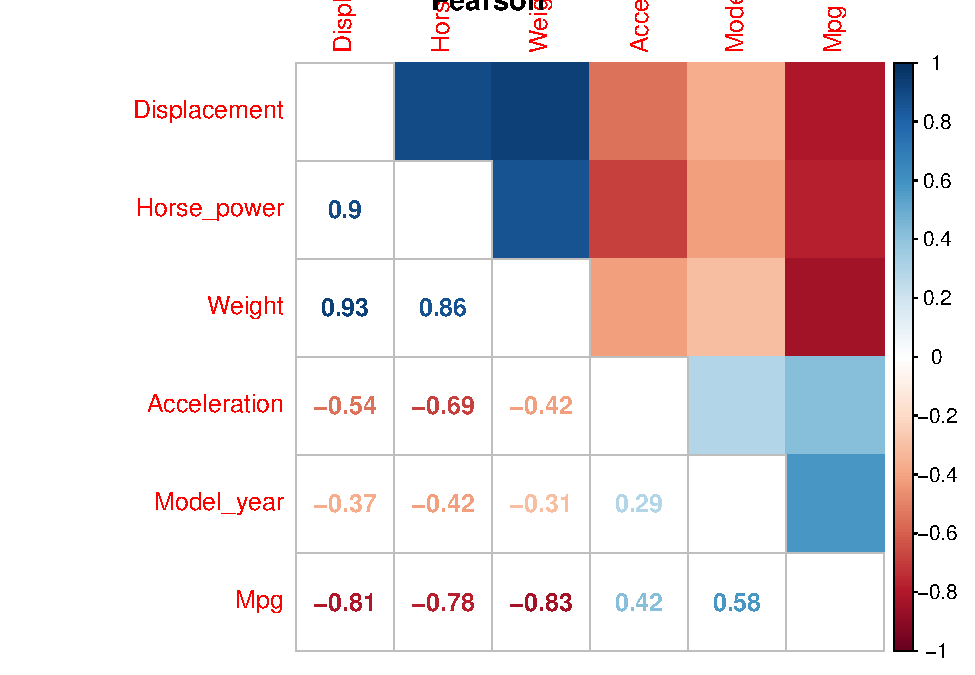
\includegraphics[width=.9\linewidth]{img/Regresion_files/figure-latex/unnamed-chunk-3-1} \caption{}\end{figure}

\begin{figure}[H]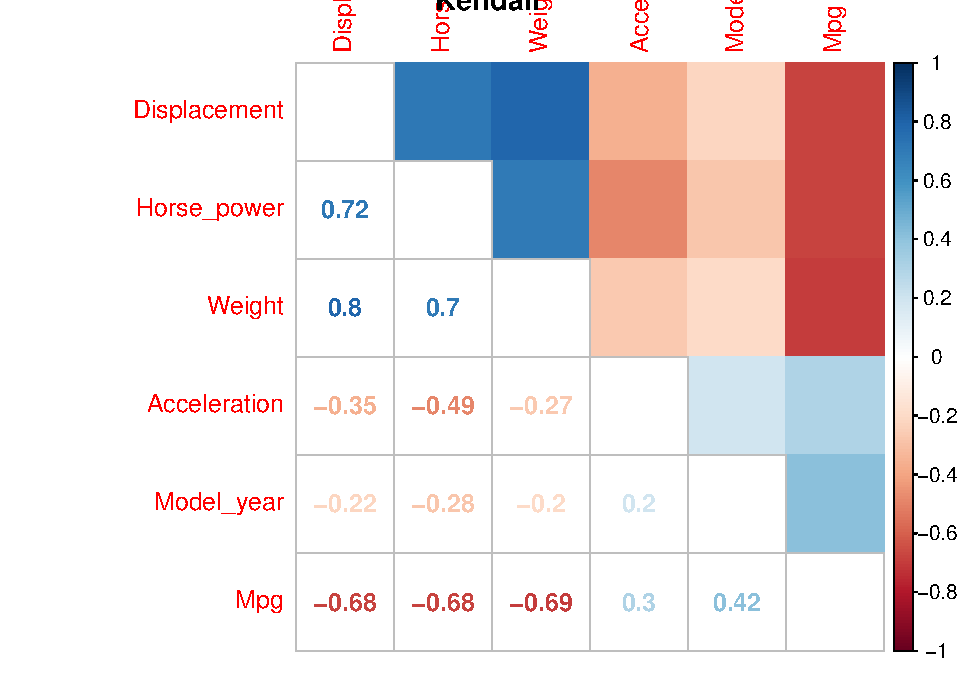
\includegraphics[width=.9\linewidth]{img/Regresion_files/figure-latex/unnamed-chunk-3-2} \caption{}\end{figure}

Por tanto, si las ordenáramos por cuáles parecen ser más prometedoras, tendríamos: Weight \textgreater{} Displacement \textgreater{} Horse\_power \textgreater{} Model\_year \textgreater{} Acceleration

También tenemos que tener en cuenta que las tres primeras variables están correladas entre sí.

\subsection{Ajustes de regresión lineal univariables}

Vamos a analizar un ajuste con cada una de las características:

\begin{verbatim}

Call: lm(formula = Mpg ~ Weight, data = auto)

Residuals:
     Min       1Q   Median       3Q      Max 
-11.9736  -2.7556  -0.3358   2.1379  16.5194 

Coefficients:
             Estimate Std. Error t value Pr(>|t|)    
(Intercept) 46.216524   0.798673   57.87   <2e-16 ***
Weight      -0.007647   0.000258  -29.64   <2e-16 ***
---
Signif. codes:  0 '***' 0.001 '**' 0.01 '*' 0.05 '.' 0.1 ' ' 1

Residual standard error: 4.333 on 390 degrees of freedom
Multiple R-squared:  0.6926,    Adjusted R-squared:  0.6918 
F-statistic: 878.8 on 1 and 390 DF,  p-value: < 2.2e-16

"-------------------------------------------"

Call: lm(formula = Mpg ~ Displacement, data = auto)

Residuals:
     Min       1Q   Median       3Q      Max 
-12.9170  -3.0243  -0.5021   2.3512  18.6128 

Coefficients:
             Estimate Std. Error t value Pr(>|t|)    
(Intercept)  35.12064    0.49443   71.03   <2e-16 ***
Displacement -0.06005    0.00224  -26.81   <2e-16 ***
---
Signif. codes:  0 '***' 0.001 '**' 0.01 '*' 0.05 '.' 0.1 ' ' 1

Residual standard error: 4.635 on 390 degrees of freedom
Multiple R-squared:  0.6482,    Adjusted R-squared:  0.6473 
F-statistic: 718.7 on 1 and 390 DF,  p-value: < 2.2e-16

"-------------------------------------------"

Call: lm(formula = Mpg ~ Horse_power, data = auto)

Residuals:
     Min       1Q   Median       3Q      Max 
-13.5710  -3.2592  -0.3435   2.7630  16.9240 

Coefficients:
             Estimate Std. Error t value Pr(>|t|)    
(Intercept) 39.935861   0.717499   55.66   <2e-16 ***
Horse_power -0.157845   0.006446  -24.49   <2e-16 ***
---
Signif. codes:  0 '***' 0.001 '**' 0.01 '*' 0.05 '.' 0.1 ' ' 1

Residual standard error: 4.906 on 390 degrees of freedom
Multiple R-squared:  0.6059,    Adjusted R-squared:  0.6049 
F-statistic: 599.7 on 1 and 390 DF,  p-value: < 2.2e-16

"-------------------------------------------"

Call: lm(formula = Mpg ~ Model_year, data = auto)

Residuals:
     Min       1Q   Median       3Q      Max 
-12.0212  -5.4411  -0.4412   4.9739  18.2088 

Coefficients:
             Estimate Std. Error t value Pr(>|t|)    
(Intercept) -70.01167    6.64516  -10.54   <2e-16 ***
Model_year    1.23004    0.08736   14.08   <2e-16 ***
---
Signif. codes:  0 '***' 0.001 '**' 0.01 '*' 0.05 '.' 0.1 ' ' 1

Residual standard error: 6.363 on 390 degrees of freedom
Multiple R-squared:  0.337, Adjusted R-squared:  0.3353 
F-statistic: 198.3 on 1 and 390 DF,  p-value: < 2.2e-16

"-------------------------------------------"

Call: lm(formula = Mpg ~ Acceleration, data = auto)

Residuals:
    Min      1Q  Median      3Q     Max 
-17.989  -5.616  -1.199   4.801  23.239 

Coefficients:
             Estimate Std. Error t value Pr(>|t|)    
(Intercept)    4.8332     2.0485   2.359   0.0188 *  
Acceleration   1.1976     0.1298   9.228   <2e-16 ***
---
Signif. codes:  0 '***' 0.001 '**' 0.01 '*' 0.05 '.' 0.1 ' ' 1

Residual standard error: 7.08 on 390 degrees of freedom
Multiple R-squared:  0.1792,    Adjusted R-squared:  0.1771 
F-statistic: 85.15 on 1 and 390 DF,  p-value: < 2.2e-16
\end{verbatim}

Al ser univariable, por ahora no es necesario fijarse en el estadístico F. Para ver el potencial de la variable, debemos darle importancia al p-valor (comprobar de que sea lo suficientemente bajo), y posteriormente ver el R\textsuperscript{2} para everiguar el porcentaje de la salida explicada.

\vspace{\baselineskip}

En base a los resultados vemos que el test de correlación nos había ayudado correctamente: de forma individual todas las variables tienen dependencia lineal, y el orden de calidad coincide con el orden de fuerza en las correlaciones.

Ya con el uso de la variable Weight vemos que podemos explicar un \textasciitilde69\% de la salida, un buen valor de partida. El ajuste quedaría de esta manera:

\begin{figure}[H]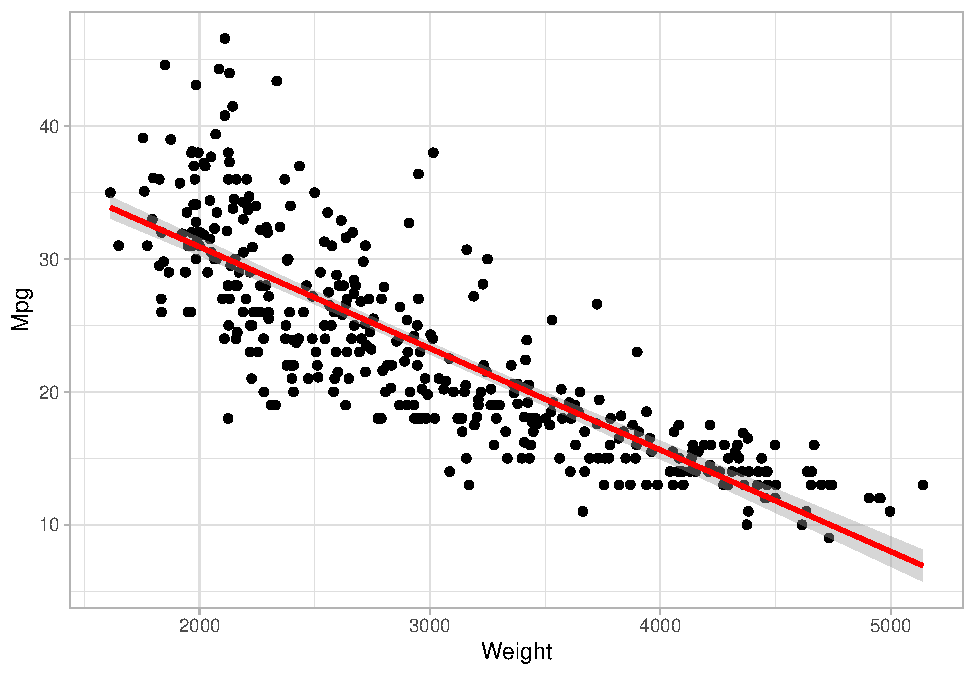
\includegraphics[width=.9\linewidth]{img/Regresion_files/figure-latex/unnamed-chunk-6-1} \caption{}\end{figure}

Con los coeficientes:

\begin{verbatim}
                   2.5 %      97.5 %
(Intercept) 44.646282308 47.78676679
Weight      -0.008154515 -0.00714017
\end{verbatim}

Aunque los valores del intervalo del coeficiente de Weight sea bajo, vemos que no incluye el cero (y con el p-valor obtenido anteriormente, lo podemos asegurar con bastante certeza). Probablemente la razón de estos coeficientes tan pequeños es que los datos no están estandarizados (se podría hacer perfectamente, se han dejado con sus rangos normales para interpretarlos mejor) y los valores de las unidades de medida son bastante diferentes (hablamos de rangos de {[}9.0,46.6{]} en Mpg frente a {[}1613,5140{]} en Weight)

\vspace{\baselineskip}

Ya con esto podemos intentan interpretar un poco los datos, tendríamos por ahora la fórmula de regresión lineal: 

\begin{equation}    
    Mpg \sim Weight
\end{equation}

\subsection{Ajustes de regresión lineal multivariable}

Aplicamos un método descendente:

\begin{verbatim}
Call: lm(formula = Mpg ~ ., data = auto)

Residuals:
    Min      1Q  Median      3Q     Max 
-8.5211 -2.3920 -0.1036  2.0312 14.2874 

Coefficients:
               Estimate Std. Error t value Pr(>|t|)    
(Intercept)  -1.544e+01  4.677e+00  -3.300  0.00106 ** 
Displacement  2.782e-03  5.462e-03   0.509  0.61082    
Horse_power   1.020e-03  1.376e-02   0.074  0.94095    
Weight       -6.874e-03  6.653e-04 -10.333  < 2e-16 ***
Acceleration  9.032e-02  1.019e-01   0.886  0.37599    
Model_year    7.541e-01  5.261e-02  14.334  < 2e-16 ***
---
Signif. codes:  0 '***' 0.001 '**' 0.01 '*' 0.05 '.' 0.1 ' ' 1

Residual standard error: 3.435 on 386 degrees of freedom
Multiple R-squared:  0.8088,    Adjusted R-squared:  0.8063 
F-statistic: 326.5 on 5 and 386 DF,  p-value: < 2.2e-16
\end{verbatim}

% \begin{center}\rule{\linewidth}{0.5pt}\end{center}

El p-valor del F estadístico nos dice que al menos hay una variable (realmente ya lo sabíamos de los ajustes univariables) con dependencia linea.

\vspace{\baselineskip}

Vemos que hay 3 variables con mal p-valor, empezamos quitando la que lo tiene más alto, Horse\_power.

\begin{center}\rule{\linewidth}{0.5pt}\end{center}

\begin{verbatim}
Call: lm(formula = Mpg ~ . - Horse_power, data = auto)

Residuals:
    Min      1Q  Median      3Q     Max 
-8.5182 -2.3948 -0.1085  2.0405 14.2908 

Coefficients:
               Estimate Std. Error t value Pr(>|t|)    
(Intercept)  -1.527e+01  4.106e+00  -3.719 0.000229 ***
Displacement  2.874e-03  5.310e-03   0.541 0.588651    
Weight       -6.852e-03  5.967e-04 -11.483  < 2e-16 ***
Acceleration  8.555e-02  7.885e-02   1.085 0.278595    
Model_year    7.532e-01  5.118e-02  14.717  < 2e-16 ***
---
Signif. codes:  0 '***' 0.001 '**' 0.01 '*' 0.05 '.' 0.1 ' ' 1

Residual standard error: 3.431 on 387 degrees of freedom
Multiple R-squared:  0.8088,    Adjusted R-squared:  0.8068 
F-statistic: 409.2 on 4 and 387 DF,  p-value: < 2.2e-16
\end{verbatim}

El F estadístico está correcto, y seguimos teniendo variables con p-valor grande, quitamos Displacement.

\begin{center}\rule{\linewidth}{0.5pt}\end{center}

\begin{verbatim}
Call: lm(formula = Mpg ~ . - Horse_power - Displacement, data = auto)

Residuals:
    Min      1Q  Median      3Q     Max 
-8.6749 -2.3528 -0.1082  2.0168 14.3022 

Coefficients:
               Estimate Std. Error t value Pr(>|t|)    
(Intercept)  -14.936555   4.055512  -3.683 0.000263 ***
Weight        -0.006554   0.000230 -28.502  < 2e-16 ***
Acceleration   0.066359   0.070361   0.943 0.346204    
Model_year     0.748446   0.050366  14.860  < 2e-16 ***
---
Signif. codes:  0 '***' 0.001 '**' 0.01 '*' 0.05 '.' 0.1 ' ' 1

Residual standard error: 3.428 on 388 degrees of freedom
Multiple R-squared:  0.8086,    Adjusted R-squared:  0.8071 
F-statistic: 546.5 on 3 and 388 DF,  p-value: < 2.2e-16
\end{verbatim}

\textit{idem}. a lo anterior, quitamos Acceleration.

\begin{center}\rule{\linewidth}{0.5pt}\end{center}

\begin{verbatim}
Call: lm(formula = Mpg ~ . - Horse_power - Displacement - Acceleration, 
    data = auto)

Residuals:
    Min      1Q  Median      3Q     Max 
-8.8505 -2.3014 -0.1167  2.0367 14.3555 

Coefficients:
              Estimate Std. Error t value Pr(>|t|)    
(Intercept) -1.435e+01  4.007e+00  -3.581 0.000386 ***
Weight      -6.632e-03  2.146e-04 -30.911  < 2e-16 ***
Model_year   7.573e-01  4.947e-02  15.308  < 2e-16 ***
---
Signif. codes:  0 '***' 0.001 '**' 0.01 '*' 0.05 '.' 0.1 ' ' 1

Residual standard error: 3.427 on 389 degrees of freedom
Multiple R-squared:  0.8082,    Adjusted R-squared:  0.8072 
F-statistic: 819.5 on 2 and 389 DF,  p-value: < 2.2e-16
\end{verbatim}

El estadístico F sigue bien, y los p-valores de las variables son extremadamente bajos. Nos fijamos en el R\textsuperscript{2} y vemos que ha subido considerablemente (un 10\%) respecto al univariable, por lo que este sería nuestro modelo aditivo por ahora.

\vspace{\baselineskip}

A partir de ahora deberíamos tener cuidado si el R\textsuperscript{2} sigue aumentando, hay que evitar el overfitting en el modelo.

\subsection{Inserción de interacciones}

Del modelo aditivo solo nos han quedado dos regresores, así que probamos a incluirlos como interacción.

\begin{verbatim}
Call: lm(formula = Mpg ~ +Weight * Model_year, data = auto)

Residuals:
    Min      1Q  Median      3Q     Max 
-8.0397 -1.9956 -0.0983  1.6525 12.9896 

Coefficients:
                    Estimate Std. Error t value Pr(>|t|)    
(Intercept)       -1.105e+02  1.295e+01  -8.531 3.30e-16 ***
Weight             2.755e-02  4.413e-03   6.242 1.14e-09 ***
Model_year         2.040e+00  1.718e-01  11.876  < 2e-16 ***
Weight:Model_year -4.579e-04  5.907e-05  -7.752 8.02e-14 ***
---
Signif. codes:  0 '***' 0.001 '**' 0.01 '*' 0.05 '.' 0.1 ' ' 1

Residual standard error: 3.193 on 388 degrees of freedom
Multiple R-squared:  0.8339,    Adjusted R-squared:  0.8326 
F-statistic: 649.3 on 3 and 388 DF,  p-value: < 2.2e-16
\end{verbatim}

El F estadístico sigue bien y los p-valores son bajos, el nuevo R\textsuperscript{2} ha mejorado un 3\%, así que no es demasiado para considerar un overfitting. Probablemente más de un 90\% sería preocupante, pero también tenemos que tener en cuenta que las variables están fuertemente correladas con la salida.

\vspace{\baselineskip}

Podríamos probar a añadir alguna interacción más con alguna variable que no hubiera entrado en el modelo aditivo, pero no se espera que mejore:

\begin{center}\rule{\linewidth}{0.5pt}\end{center}

\begin{verbatim}
Call: lm(formula = Mpg ~ +Weight * Model_year + Acceleration * Displacement, 
    data = auto)

Residuals:
    Min      1Q  Median      3Q     Max 
-7.3130 -1.8670 -0.0426  1.6109 12.2499 

Coefficients:
                            Estimate Std. Error t value Pr(>|t|)    
(Intercept)               -1.131e+02  1.321e+01  -8.564 2.65e-16 ***
Weight                     2.456e-02  4.693e-03   5.234 2.73e-07 ***
Model_year                 1.907e+00  1.769e-01  10.778  < 2e-16 ***
Acceleration               7.273e-01  1.282e-01   5.671 2.79e-08 ***
Displacement               3.605e-02  8.673e-03   4.157 3.98e-05 ***
Weight:Model_year         -4.054e-04  6.281e-05  -6.454 3.29e-10 ***
Acceleration:Displacement -2.953e-03  6.219e-04  -4.748 2.91e-06 ***
---
Signif. codes:  0 '***' 0.001 '**' 0.01 '*' 0.05 '.' 0.1 ' ' 1

Residual standard error: 3.075 on 385 degrees of freedom
Multiple R-squared:  0.8472,    Adjusted R-squared:  0.8448 
F-statistic: 355.7 on 6 and 385 DF,  p-value: < 2.2e-16
\end{verbatim}

A pesar de nuestra suposición los p-valores son válidos y el R\textsuperscript{2} aumenta un 1\%. Es cuestionable si el aumento de la complejidad del modelo merece con este incremento de R\textsuperscript{2}. Por simplificar vamos a quedarnos con el modelo aditivo anterior y probar con otra interacción.

\vspace{\baselineskip}

Podemos probar combinando la variable Acceleration separadamente con las que ya teníamos (Weight y Model\_year).

\begin{center}\rule{\linewidth}{0.5pt}\end{center}

\begin{verbatim}

Call: lm(formula = Mpg ~ +Weight * Model_year + Acceleration * Weight, 
    data = auto)

Residuals:
    Min      1Q  Median      3Q     Max 
-7.4473 -1.7994 -0.0496  1.4790 12.1258 

Coefficients:
                      Estimate Std. Error t value Pr(>|t|)    
(Intercept)         -1.230e+02  1.298e+01  -9.480  < 2e-16 ***
Weight               2.971e-02  4.419e-03   6.722 6.47e-11 ***
Model_year           1.926e+00  1.742e-01  11.055  < 2e-16 ***
Acceleration         1.341e+00  2.323e-01   5.772 1.61e-08 ***
Weight:Model_year   -4.078e-04  6.197e-05  -6.581 1.53e-10 ***
Weight:Acceleration -3.808e-04  7.537e-05  -5.052 6.76e-07 ***
---
Signif. codes:  0 '***' 0.001 '**' 0.01 '*' 0.05 '.' 0.1 ' ' 1

Residual standard error: 3.061 on 386 degrees of freedom
Multiple R-squared:  0.8482,    Adjusted R-squared:  0.8462 
F-statistic: 431.4 on 5 and 386 DF,  p-value: < 2.2e-16
\end{verbatim}

\begin{center}\rule{\linewidth}{0.5pt}\end{center}

\begin{verbatim}
Call: lm(formula = Mpg ~ +Weight * Model_year + Acceleration * Model_year, 
    data = auto)

Residuals:
    Min      1Q  Median      3Q     Max 
-7.8674 -1.9539 -0.0617  1.7397 12.3964 

Coefficients:
                          Estimate Std. Error t value Pr(>|t|)    
(Intercept)             -4.046e+01  2.833e+01  -1.428  0.15401    
Weight                   2.523e-02  4.881e-03   5.170 3.76e-07 ***
Model_year               1.072e+00  3.704e-01   2.895  0.00401 ** 
Acceleration            -3.956e+00  1.268e+00  -3.120  0.00195 ** 
Weight:Model_year       -4.263e-04  6.475e-05  -6.584 1.49e-10 ***
Model_year:Acceleration  5.476e-02  1.663e-02   3.293  0.00108 ** 
---
Signif. codes:  0 '***' 0.001 '**' 0.01 '*' 0.05 '.' 0.1 ' ' 1

Residual standard error: 3.117 on 386 degrees of freedom
Multiple R-squared:  0.8426,    Adjusted R-squared:  0.8406 
F-statistic: 413.2 on 5 and 386 DF,  p-value: < 2.2e-16
\end{verbatim}

Y entre los dos nos podríamos quedar con el primero por tener mejores p-valores y un mejor R\textsuperscript{2}. Aun así, el incremento es pequeño respecto a nuestro modelo aditivo.

\vspace{\baselineskip}

La fórmula del modelo aditivo que llevamos por ahora es:
\begin{equation}
    Mpg \sim Weight + Model_year + Acceleration + Weight*Model_year + Weight*Acceleration
\end{equation}

Gráficamente:
\begin{figure}[H]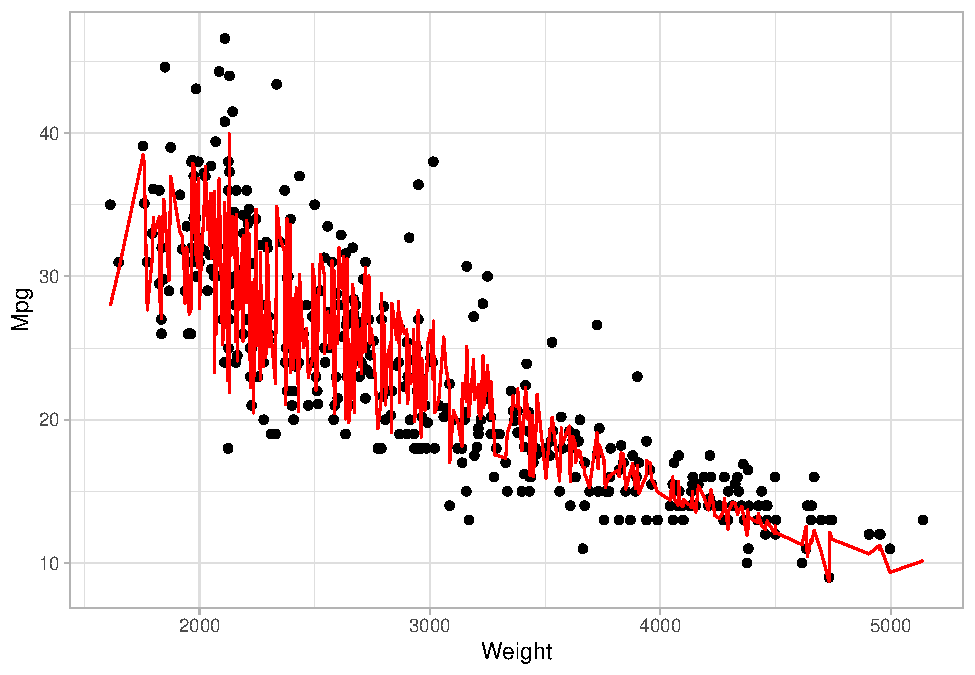
\includegraphics[width=.9\linewidth]{img/Regresion_files/figure-latex/unnamed-chunk-16-1} \caption{}\end{figure}

Por el uso multivariable la línea de regresión que se forma podría indicarnos un posible overfitting en el modelo, vamos a dejarlo por ahora e intentar solucionarlo con el modelo no lineal.

\subsection{Ajustes de regresión no lineal}

Habíamos dicho que las gráficas nos mostraban una tendencia logarítmica, vamos a incluír la de Weight en nuestro modelo aditivo:
\begin{verbatim}
Call: lm(formula = Mpg ~ +Weight * Model_year + Acceleration * Weight + 
    I(log(Weight)), data = auto)

Residuals:
    Min      1Q  Median      3Q     Max 
-7.6734 -1.7933 -0.0576  1.3154 12.1716 

Coefficients:
                      Estimate Std. Error t value Pr(>|t|)    
(Intercept)          1.191e+02  4.120e+01   2.891  0.00406 ** 
Weight               2.842e-02  4.227e-03   6.723 6.44e-11 ***
Model_year           1.638e+00  1.728e-01   9.480  < 2e-16 ***
Acceleration         7.236e-01  2.435e-01   2.972  0.00315 ** 
I(log(Weight))      -3.028e+01  4.914e+00  -6.162 1.81e-09 ***
Weight:Model_year   -2.971e-04  6.186e-05  -4.803 2.24e-06 ***
Weight:Acceleration -1.775e-04  7.919e-05  -2.241  0.02559 *  
---
Signif. codes:  0 '***' 0.001 '**' 0.01 '*' 0.05 '.' 0.1 ' ' 1

Residual standard error: 2.924 on 385 degrees of freedom
Multiple R-squared:  0.8618,    Adjusted R-squared:  0.8597 
F-statistic: 400.2 on 6 and 385 DF,  p-value: < 2.2e-16
\end{verbatim}

El estadístico F está bien y los p-valores también, aunque el de la interacción Weight-Acceleration es alto comparado con el resto (aún así sigue siendo aceptable).

Como el R\textsuperscript{2} ha subido, por ver si mejora, vamos a quitar esta interacción.

\begin{center}\rule{\linewidth}{0.5pt}\end{center}

\begin{verbatim}
Call: lm(formula = Mpg ~ +Weight * Model_year + I(log(Weight)), data = auto)

Residuals:
    Min      1Q  Median      3Q     Max 
-8.7501 -1.7470 -0.0725  1.3122 12.6776 

Coefficients:
                    Estimate Std. Error t value Pr(>|t|)    
(Intercept)        1.715e+02  3.810e+01   4.501 8.98e-06 ***
Weight             2.522e-02  4.119e-03   6.123 2.25e-09 ***
Model_year         1.572e+00  1.708e-01   9.202  < 2e-16 ***
I(log(Weight))    -3.540e+01  4.538e+00  -7.800 5.82e-14 ***
Weight:Model_year -2.701e-04  6.003e-05  -4.499 9.04e-06 ***
---
Signif. codes:  0 '***' 0.001 '**' 0.01 '*' 0.05 '.' 0.1 ' ' 1

Residual standard error: 2.972 on 387 degrees of freedom
Multiple R-squared:  0.8565,    Adjusted R-squared:  0.855 
F-statistic: 577.3 on 4 and 387 DF,  p-value: < 2.2e-16
\end{verbatim}

Hemos empeorado un 0.5\%, bastante poco, y el modelo es más simple. La dejamos quitada.

Mostramos este ajuste:
\begin{figure}[H]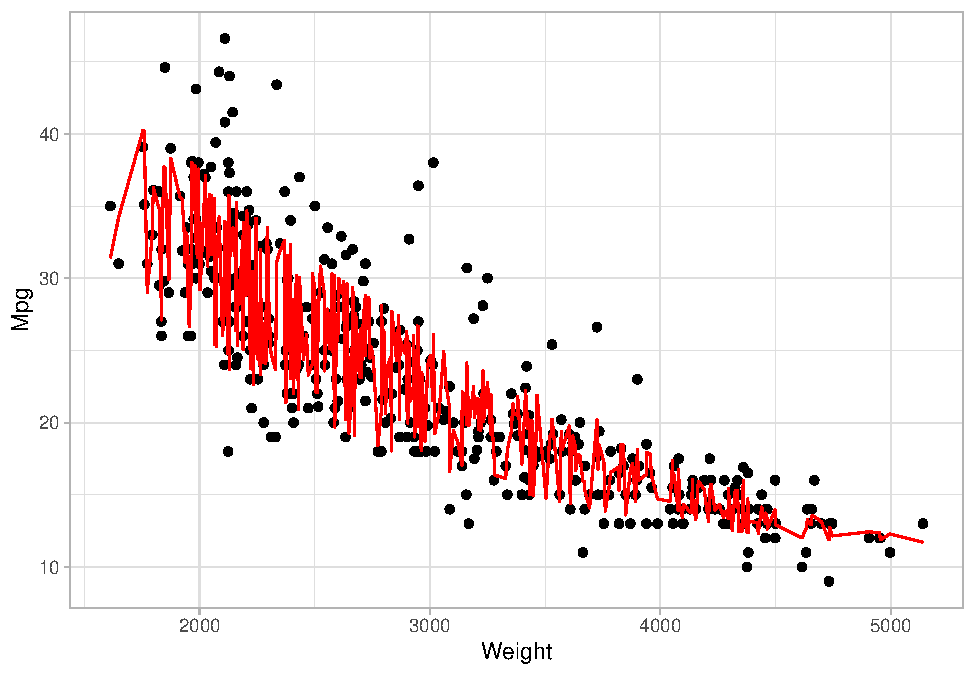
\includegraphics[width=.9\linewidth]{img/Regresion_files/figure-latex/unnamed-chunk-19-1} \caption{}\end{figure}

Esta gráfica nos indica que es probable que se esté generando sobreajuste, se ve necesario simplificar el modelo.

\begin{center}\rule{\linewidth}{0.5pt}\end{center}

Si quitamos la otra interacción:
\begin{verbatim}

Call: lm(formula = Mpg ~ Weight + Model_year + I(log(Weight)), data = auto)

Residuals:
    Min      1Q  Median      3Q     Max 
-9.3384 -1.7476 -0.2122  1.5322 13.2812 

Coefficients:
                 Estimate Std. Error t value Pr(>|t|)    
(Intercept)    284.287315  29.392946   9.672  < 2e-16 ***
Weight           0.007772   0.001420   5.473 7.97e-08 ***
Model_year       0.828693   0.044506  18.620  < 2e-16 ***
I(log(Weight)) -43.590633   4.258803 -10.235  < 2e-16 ***
---
Signif. codes:  0 '***' 0.001 '**' 0.01 '*' 0.05 '.' 0.1 ' ' 1

Residual standard error: 3.045 on 388 degrees of freedom
Multiple R-squared:  0.849, Adjusted R-squared:  0.8478 
F-statistic:   727 on 3 and 388 DF,  p-value: < 2.2e-16
\end{verbatim}

No hemos perdido apenas R\textsuperscript{2}. Mostramos la gráfica:

\begin{figure}[H]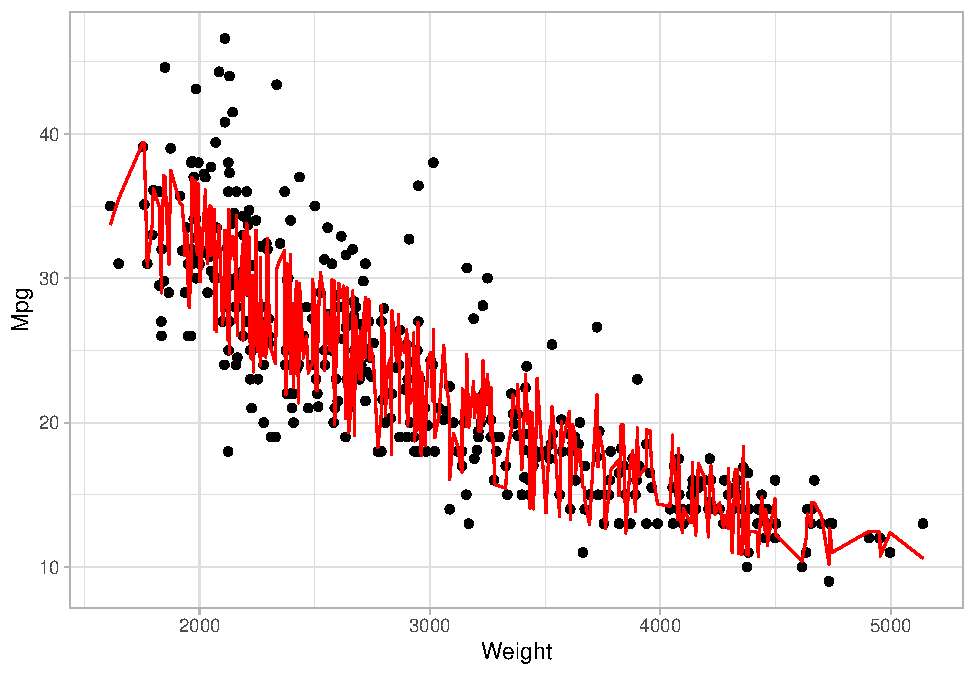
\includegraphics[width=.9\linewidth]{img/Regresion_files/figure-latex/unnamed-chunk-21-1} \caption{}\end{figure}

Seguimos con el mismo problema, probablemente se deba a una de las variables. Quitamos Model\_year por tener poca correlación con la variable de salida:

\begin{verbatim}
Call: lm(formula = Mpg ~ Weight + I(log(Weight)), data = auto)

Residuals:
     Min       1Q   Median       3Q      Max 
-12.5329  -2.7031  -0.4016   1.7038  16.0835 

Coefficients:
                 Estimate Std. Error t value Pr(>|t|)    
(Intercept)    263.812407  40.366256   6.535 1.99e-10 ***
Weight           0.002582   0.001914   1.349    0.178    
I(log(Weight)) -31.166013   5.780558  -5.392 1.21e-07 ***
---
Signif. codes:  0 '***' 0.001 '**' 0.01 '*' 0.05 '.' 0.1 ' ' 1

Residual standard error: 4.185 on 389 degrees of freedom
Multiple R-squared:  0.714, Adjusted R-squared:  0.7125 
F-statistic: 485.6 on 2 and 389 DF,  p-value: < 2.2e-16
\end{verbatim}

El p-valor de Weight nos indica que hay que quitarla, y al no estar incluída ninguna interacción, no es un término de jerarquía, por lo que podemos hacerlo. Se puede porque la variable sigue siendo independiente, solamente no está modelada de forma lineal, sino logarítmicamente.

\begin{verbatim}
Call: lm(formula = Mpg ~ I(log(Weight)), data = auto)

Residuals:
     Min       1Q   Median       3Q      Max 
-12.4315  -2.6752  -0.2888   1.9429  16.0136 

Coefficients:
               Estimate Std. Error t value Pr(>|t|)    
(Intercept)    209.9433     6.0002   34.99   <2e-16 ***
I(log(Weight)) -23.4317     0.7534  -31.10   <2e-16 ***
---
Signif. codes:  0 '***' 0.001 '**' 0.01 '*' 0.05 '.' 0.1 ' ' 1

Residual standard error: 4.189 on 390 degrees of freedom
Multiple R-squared:  0.7127,    Adjusted R-squared:  0.7119 
F-statistic: 967.3 on 1 and 390 DF,  p-value: < 2.2e-16
\end{verbatim}

\begin{figure}[H]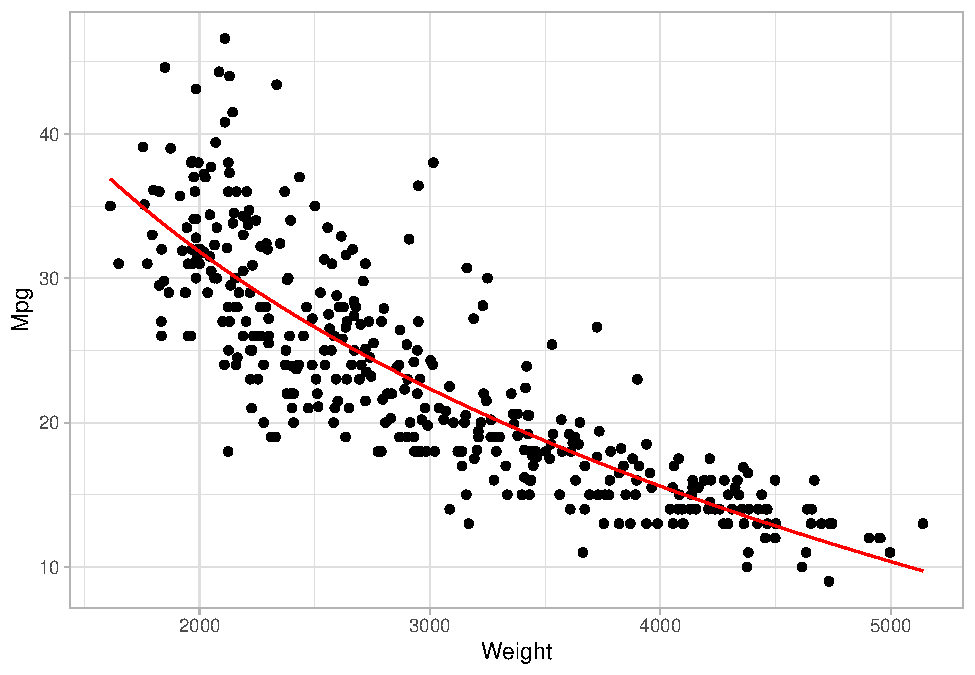
\includegraphics[width=.9\linewidth]{img/Regresion_files/figure-latex/unnamed-chunk-24-1} \caption{}\end{figure}

\begin{figure}[H]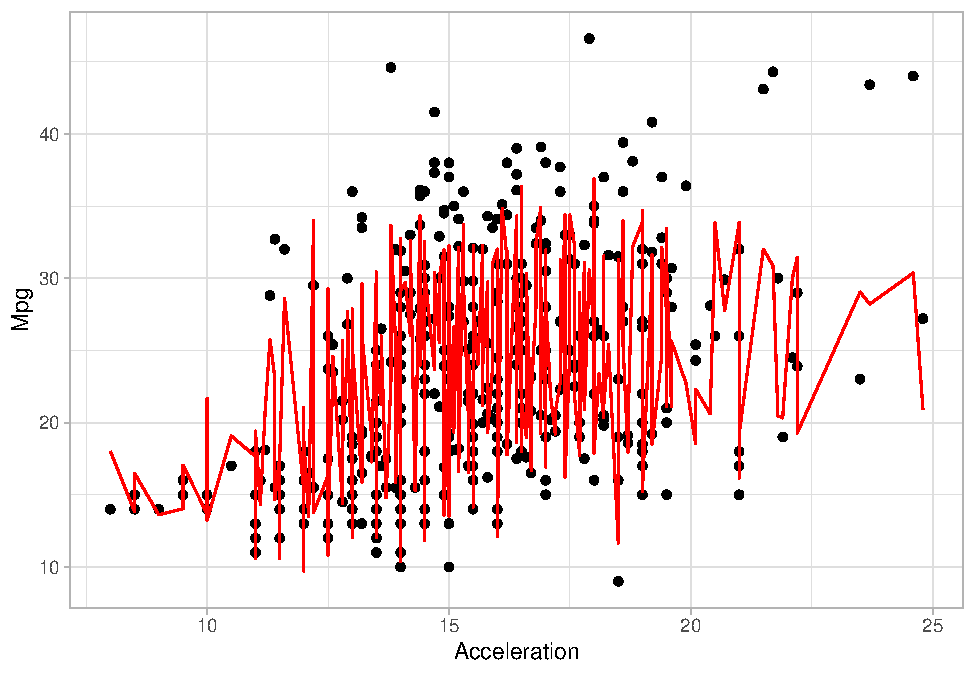
\includegraphics[width=.9\linewidth]{img/Regresion_files/figure-latex/unnamed-chunk-24-2} \caption{}\end{figure}

\begin{figure}[H]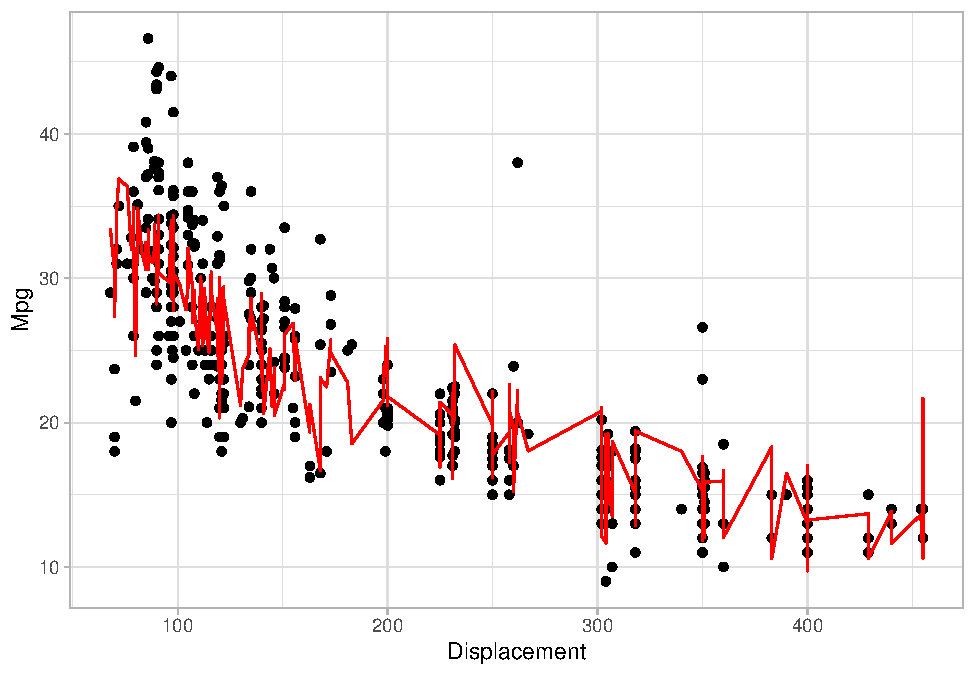
\includegraphics[width=.9\linewidth]{img/Regresion_files/figure-latex/unnamed-chunk-24-3} \caption{}\end{figure}

Vemos un empeoramiento significativo en la calidad de R\textsuperscript{2} respecto al modelo multivariable, pero la forma del modelo no está tan ajustada a los datos y parece sensato mantenerlo así.

Aún así, no resulta lógico intentar predecir el Mpg de un coche únicamente en base al peso, alguna de las otras variables deberían ayudarnos en la predicción. Por ejemplo, alguna característica del motor, como la cilindrada o los caballos de vapor.

\vspace{\baselineskip}

Para resumir, mostramos el modelo con mejor R\textsuperscript{2} tras hacer múltiples pruebas, e intentando evitar un overfitting:
\begin{verbatim}
Call: lm(formula = Mpg ~ Acceleration + I(log(Weight)) + I(log(Displacement)), 
    data = auto)

Residuals:
     Min       1Q   Median       3Q      Max 
-12.9074  -2.6174  -0.4104   1.9500  16.5596 

Coefficients:
                      Estimate Std. Error t value Pr(>|t|)    
(Intercept)          171.61778   12.14751  14.128  < 2e-16 ***
Acceleration           0.19717    0.08914   2.212   0.0276 *  
I(log(Weight))       -16.94003    2.27727  -7.439 6.59e-13 ***
I(log(Displacement))  -3.19963    1.26881  -2.522   0.0121 *  
---
Signif. codes:  0 '***' 0.001 '**' 0.01 '*' 0.05 '.' 0.1 ' ' 1

Residual standard error: 4.104 on 388 degrees of freedom
Multiple R-squared:  0.7256,    Adjusted R-squared:  0.7235 
F-statistic: 342.1 on 3 and 388 DF,  p-value: < 2.2e-16
\end{verbatim}

Los p-valores no son muy fuertes, pero siguen siendo aceptables, y gráficamente el modelo se ve un poco mejor:
\begin{figure}[H]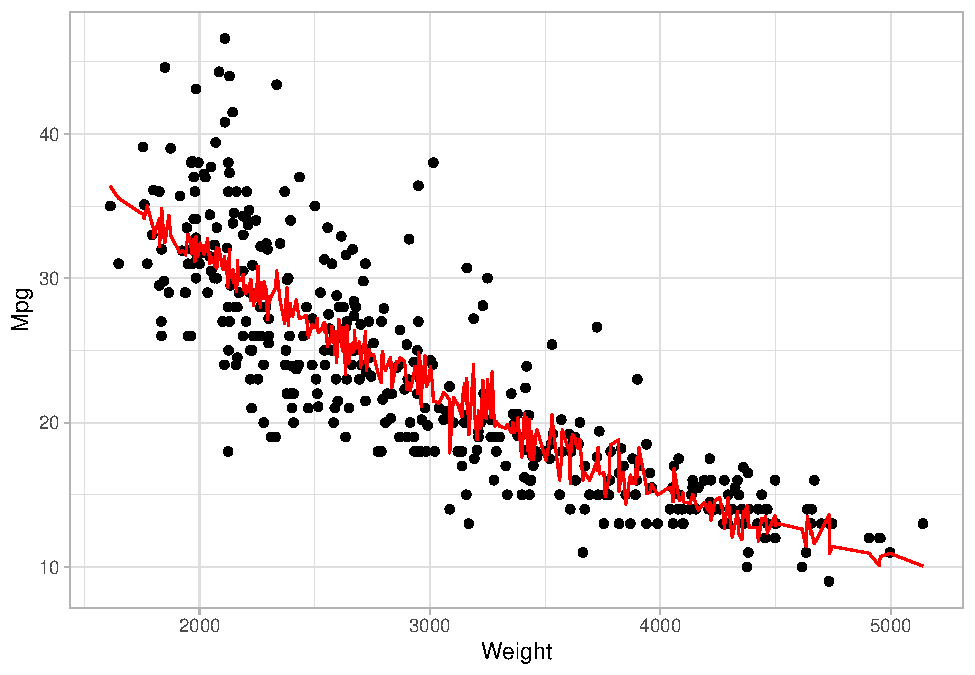
\includegraphics[width=.9\linewidth]{img/Regresion_files/figure-latex/unnamed-chunk-26-1} \caption{}\end{figure}

\begin{figure}[H]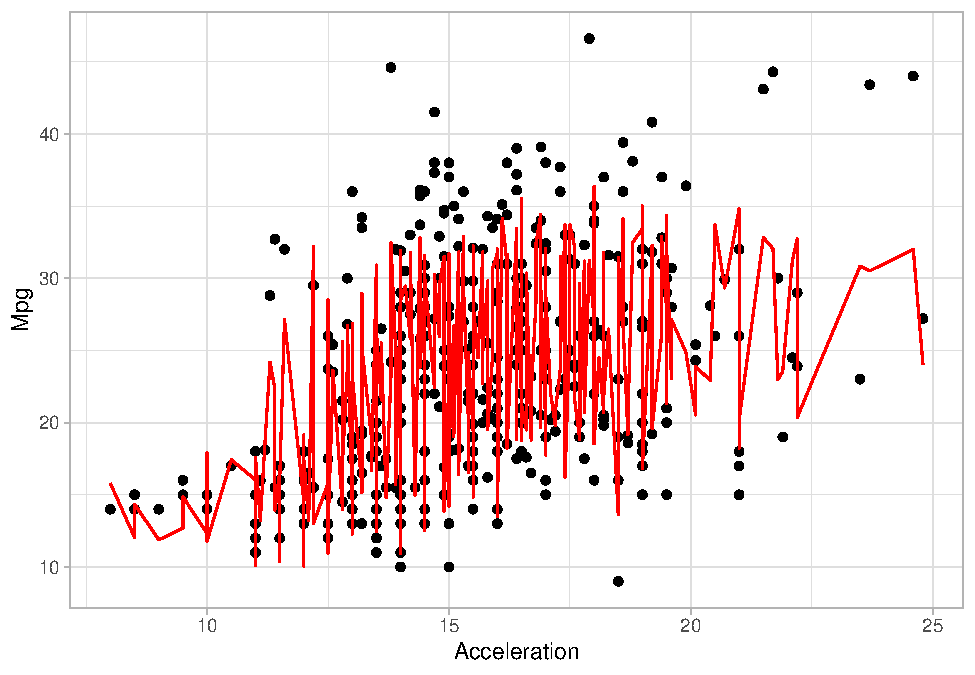
\includegraphics[width=.9\linewidth]{img/Regresion_files/figure-latex/unnamed-chunk-26-2} \caption{}\end{figure}

\begin{figure}[H]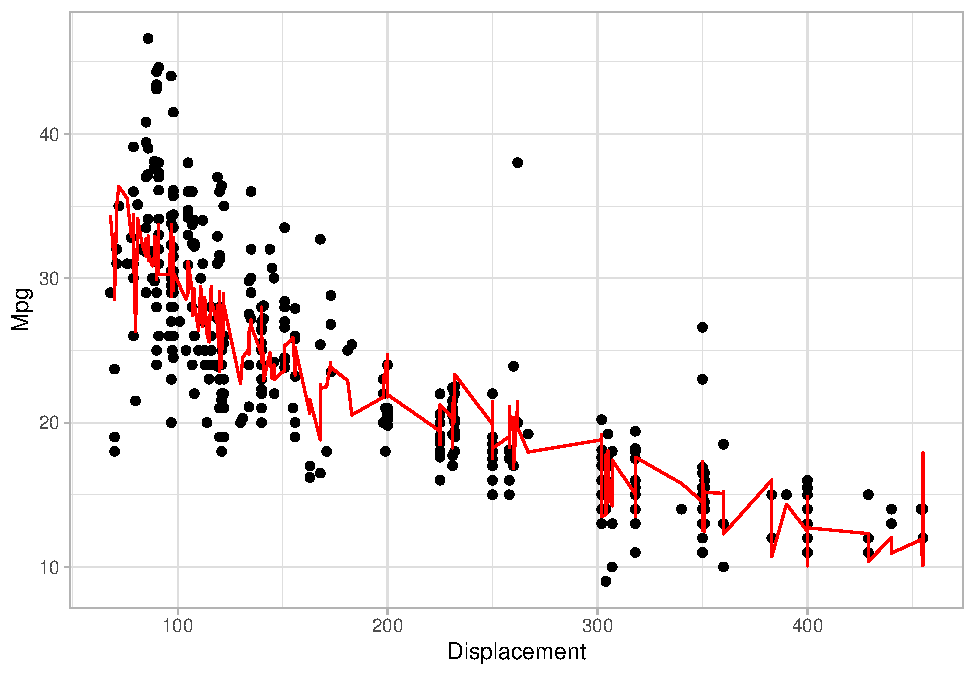
\includegraphics[width=.9\linewidth]{img/Regresion_files/figure-latex/unnamed-chunk-26-3} \caption{}\end{figure}

Pensando en el problema, y tras el análisis hecho en el apartado de EDA, creemos que usar Model\_year para predecir Mpg no parece buena idea. La gráfica de la variable nos muestra mucha dispersión en los datos y, aunque sí se ve un cierta tendencia lineal, no parece suficiente para usarla. Claramente nos ajusta mejor los datos pero parece que nos estamos pegando a ellos.

De cara a comprobar este razonamiento en el cross-validation, vamos a guardar dos modelos: 

\vspace{\baselineskip}
Modelo con mejor R\textsuperscript{2} 

\begin{equation}    
    Mpg \sim Weight + Model\_year + I(log(Weight)
\end{equation}

Modelo intentando evitar el overfitting
\begin{equation}    
    Mpg \sim Acceleration + I(log(Weight)) + I(log(Displacement))
\end{equation}

\subsection{Ajustes con KNN}

Sabemos que la función por defecto usa la distancia de Minkowski y escala los datos a igual rango. También usa un K de 7, pero sería recomendable probar con varios.

\vspace{\baselineskip}

Vamos a probar con diferentes modelos, primero el multivariable con todas
\begin{verbatim}
Mpg ~ .
    1.880835
\end{verbatim}

Y probando con varios obtenemos el menor error eliminando únicamente Acceleration:
\begin{verbatim}
Mpg ~ . - Acceleration    
    1.856269
\end{verbatim}

Que visualmente nos quedaría:
\begin{figure}[H]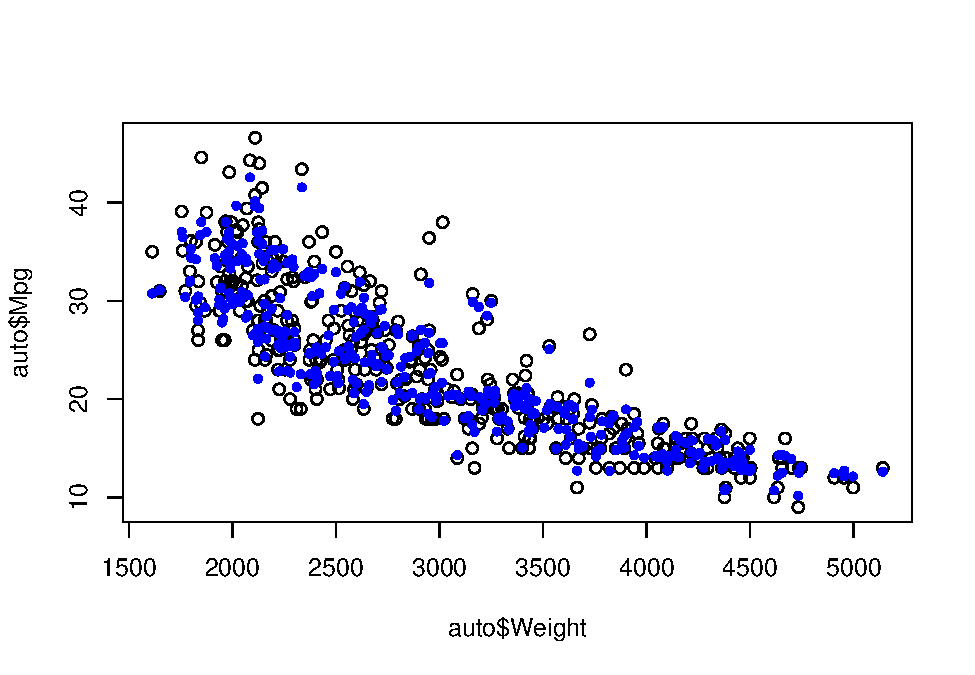
\includegraphics[width=.9\linewidth]{img/Regresion_files/figure-latex/unnamed-chunk-29-1} \caption{}\end{figure}

\begin{figure}[H]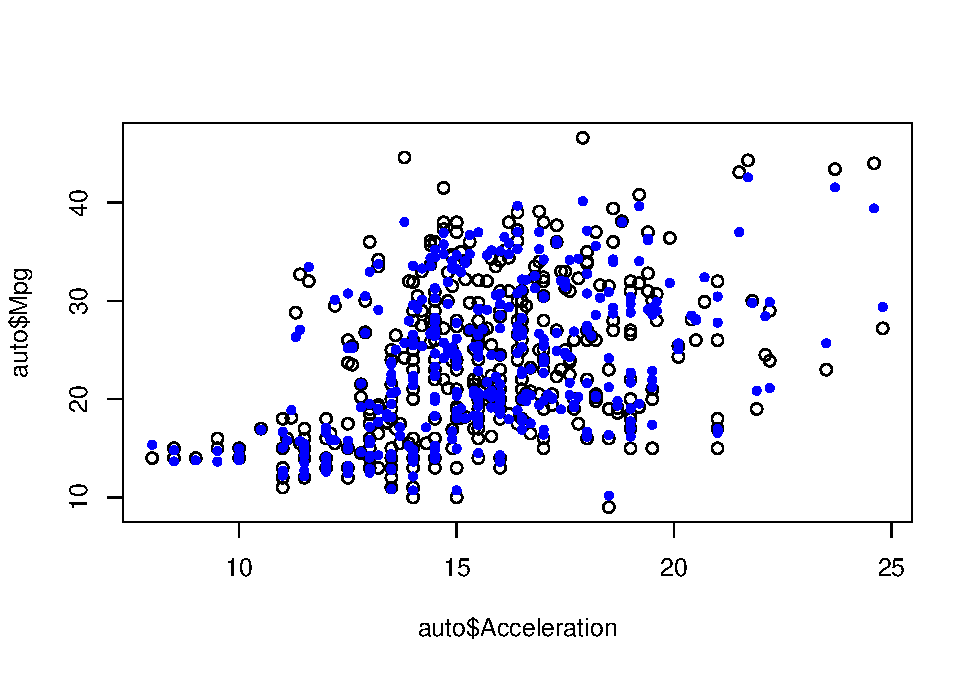
\includegraphics[width=.9\linewidth]{img/Regresion_files/figure-latex/unnamed-chunk-29-2} \caption{}\end{figure}

Si probamos el modelo no lineal obtenido en los pasos anteriores (con mejor R\textsuperscript{2}) nos un error bastante malo.
\begin{verbatim}
Mpg ~ Weight + Model_year + I(log(Weight))
    2.104086
\end{verbatim}

\vspace{\baselineskip}

El método para evitar el overfitting que usamos en el apartado anterior probablemente no funcione con KNN por seguir una metodología totalmente diferente. El ajuste de KNN para regresión no tiene nada que ver con los modelos LM. Podemos aún así comprobarlo:
\begin{verbatim}
Mpg ~ Acceleration + I(log(Weight)
    2.938051
\end{verbatim}

Gráficamente este quedaría de la siguiente manera:
\begin{figure}[H]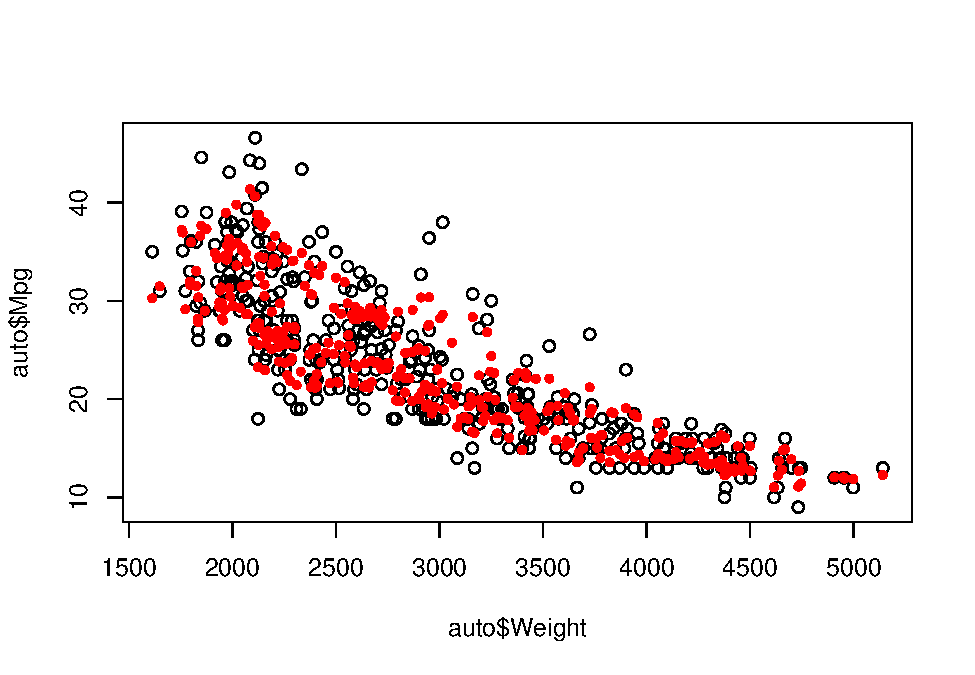
\includegraphics[width=.9\linewidth]{img/Regresion_files/figure-latex/unnamed-chunk-32-1} \caption{}\end{figure}

\begin{figure}[H]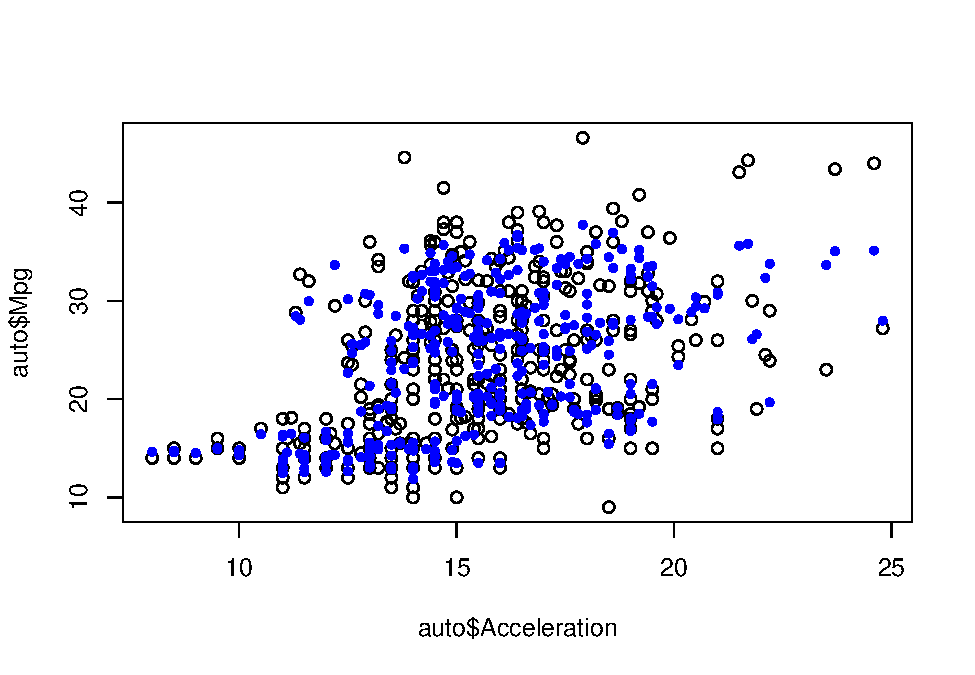
\includegraphics[width=.9\linewidth]{img/Regresion_files/figure-latex/unnamed-chunk-32-2} \caption{}\end{figure}

Por completitud, podríamos usarlo también en cross-validation para comprobarlo con un conjunto de test.

\vspace{\baselineskip}

Tendríamos por tanto los siguientes modelos para KNN: 
\begin{equation}
    Mpg \sim . - Acceleration 
\end{equation}

\begin{equation}    
    Mpg \sim Acceleration + I(log(Weight)) + I(log(Displacement))
\end{equation}

\vspace{\baselineskip}

Comparándolos gráficamente vemos que son similares, aunque el que intenta evitar el overfitting (en color azul en la gráfica), tiene menor dispersión:
\begin{figure}[H]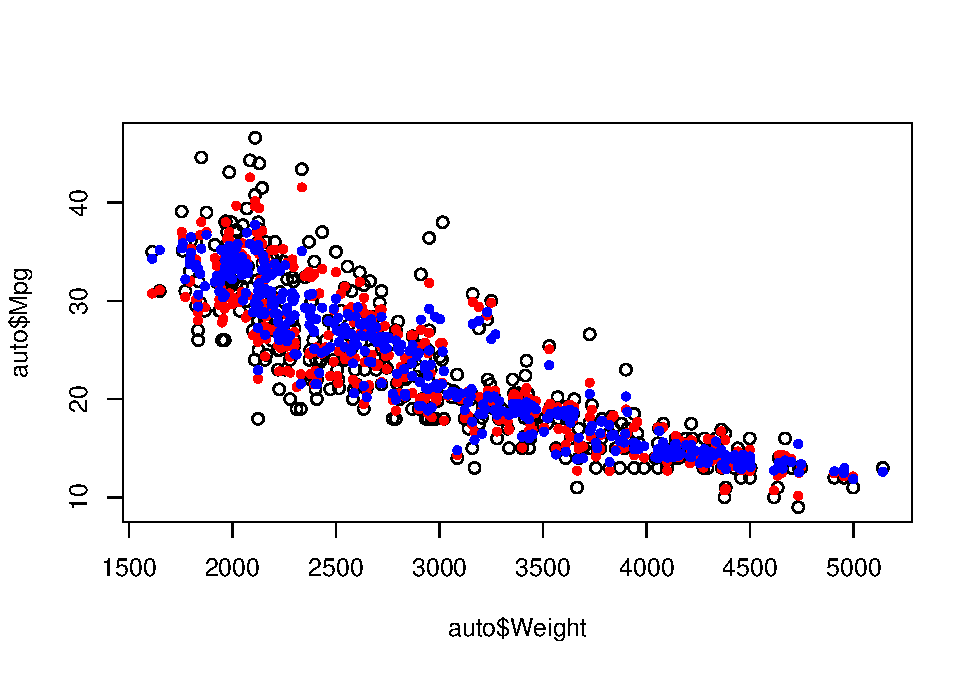
\includegraphics[width=.9\linewidth]{img/Regresion_files/figure-latex/unnamed-chunk-33-1} \caption{}\end{figure}

\begin{figure}[H]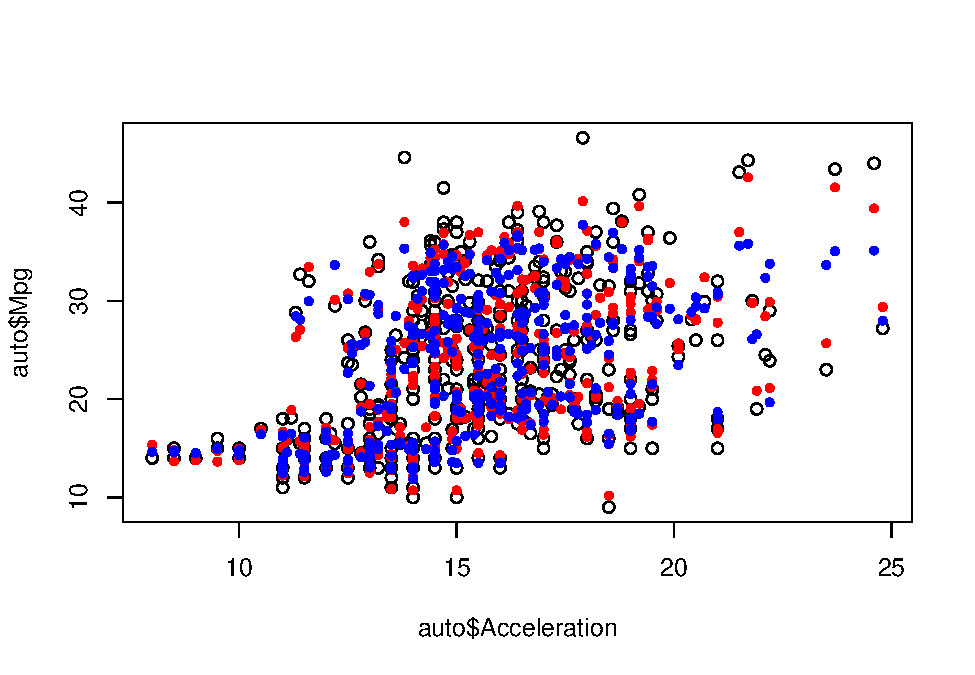
\includegraphics[width=.9\linewidth]{img/Regresion_files/figure-latex/unnamed-chunk-33-2} \caption{}\end{figure}

\subsection{Comparativa de los ajustes anteriores con cross-validation}

Recordamos los modelos obtenidos.

\vspace{\baselineskip}
LM: 
\begin{equation}
    Mpg \sim Weight + Model\_year + I(log(Weight)
\end{equation}
\begin{equation}    
    Mpg \sim Acceleration + I(log(Weight)) + I(log(Displacement))
\end{equation}

\vspace{\baselineskip}
KNN: 
\begin{equation}    
    Mpg \sim . - Acceleration
\end{equation}

\begin{equation}    
    Mpg \sim Acceleration + I(log(Weight)) + I(log(Displacement))
\end{equation}

\vspace{\baselineskip}

Con el proceso de cross-validation dividimos el dataset en N subconjuntos (folds) y repetimos el entrenamiento N veces. Cada entrenamiento se aplica reservando uno de los subconjuntos como test y entrenando con el resto. Al final, el error obtenido para el modelo es la media de los errores en cada fold. La elección del número de folds es importante y si el problema lo permite (en términos de gasto computacional), se debería probar con varios. En este caso hemos utilizado 5 folds.

Con esto conseguimos no desperdiciar el conocimiento del conjunto de test y no guiarnos por una única evaluación del modelo.

\vspace{\baselineskip}

Aplicando este proceso obtenemos los siguiente:
\begin{verbatim}
Regresión 1:  9.333066
Regresión 2: 17.10519
KNN 1:        7.291517
KNN 2:       18.43846
\end{verbatim}

Los resultados nos muestra que los modelos con los que obtuvimos mejores valores de R\textsuperscript{2} y RSME en sus apartados han acabado con mejor RSME tras el cross-validation. También apreciamos que con KNN conseguimos ligeramente mejores resultados que regresión lineal/no-lineal.

\vspace{\baselineskip}

Por completitud, mostramos también los resultados en training:
\begin{verbatim}
Regresión 1:  9.159891
Regresión 2: 16.62285
KNN 1:        3.659828
KNN 2:        8.642349
\end{verbatim}

Que nos muestran que ninguno de los modelos LM estaba haciendo overfitting. 
Adicionalmente, en KNN existe una diferencia significativa entre training y test.

\subsection{Comparativa de tests}

Para comparar los algoritmos vamos a aplicar test estadísticos en base a los resultados obtenidos en múltiples datasets. Para asegurar la igualdad de condiciones los algoritmos hacen uso de parámetros genéricos y utilizan las mismas particiones de cross-validation.

\vspace{\baselineskip}

Estas son las tablas de resultados que tenemos para test:
\begin{longtable}[]{@{}rr@{}}
\toprule
out\_test\_lm & out\_test\_kknn\tabularnewline
\midrule
\endhead
0.1909091 & 0.1000000\tabularnewline
0.1000000 & 1.0294118\tabularnewline
0.1000000 & 0.4339071\tabularnewline
0.1000000 & 0.3885965\tabularnewline
0.1548506 & 0.1000000\tabularnewline
0.1000000 & 0.3061057\tabularnewline
\bottomrule
\end{longtable}

\vspace{\baselineskip}

Aplicamos el test de Wilconxon a LM y KNN:
\begin{verbatim}
 V    V
78 - 93 

p-value:  0.7660294
\end{verbatim}

Obtenemos un ranking de 78 para LM y 93 para KNN, con un p-valor de 0.77 (o nivel de confianza del 33\%).

Esto nos dice que gana KNN pero puesto que el p-value no es lo suficientemente grande no podemos afirmar con un nivel alto de significación que las diferencias entre los tests sean notorias.

\vspace{\baselineskip}

Ahora aplicamos en test de Friedman a los dos algoritmos anteriores junto al algoritmo M5:
\begin{verbatim}
Friedman rank sum test

data:  as.matrix(tablatst)
Friedman chi-squared = 8.4444, df = 2, p-value = 0.01467
\end{verbatim}

El p-value es \textless0.05 por lo que podemos concluir que al menos hay un par de algoritmos de calidad diferente.

\vspace{\baselineskip}

Vemos cuáles de ellos lo son haciendo el test post-hoc de HOLM
\begin{verbatim}
Pairwise comparisons using Wilcoxon signed rank exact test 

data:  as.matrix(tablatst) and groups 

  1     2    
2 0.580 -    
3 0.081 0.108

P value adjustment method: holm 
\end{verbatim}

Con el test post-hoc de HOLM podemos asegurar que 3-1 (M5 vs LM) son diferentes. También podemos afirmar M5 respecto de KNN pero con un nivel de confianza menor.

\vspace{\baselineskip}

De KNN y LM no podemos afirmar nada puesto que el p-valor es extremadamente grande. \newpage
    % \section{Técnicas de Clasificación}

Como hemos visto en el apartado de EDA, tenemos un conjunto desbalanceado. Por la descripción del problema, cometemos un error mayor cuando clasificamos mal la clase Yes. Por tanto, se podría considerar penalizar más los falsos negativos, de manera que los algoritmos de clasificación intenten cometer menores errores de este tipo. 

\subsection{Algoritmo KNN}

Recordamos los gráficos 1-1 con las clasificaciones, vistos en el EDA.

\begin{figure}[H]\center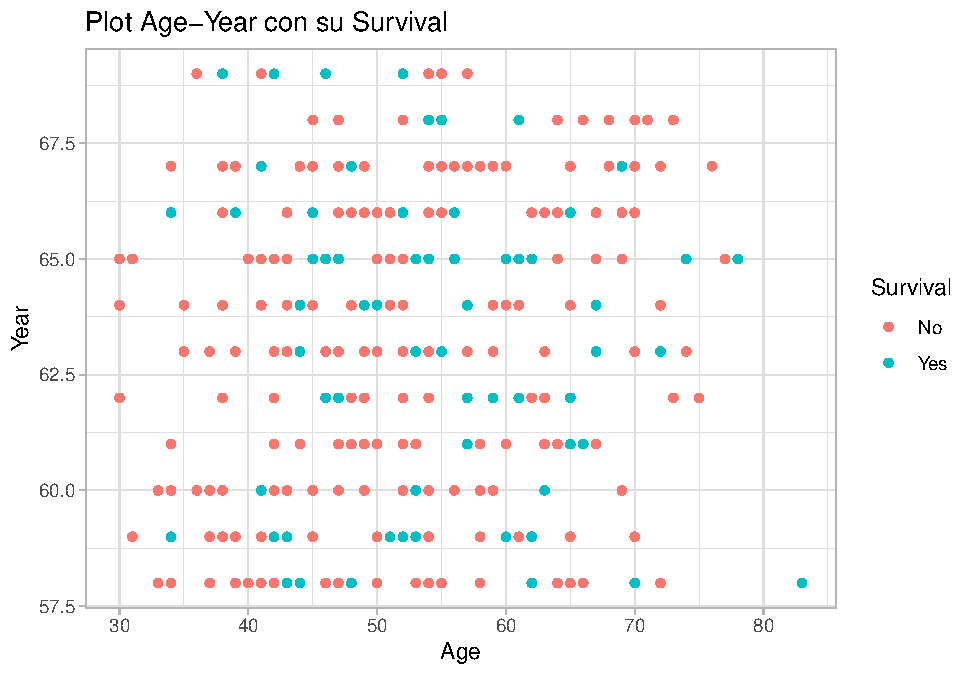
\includegraphics[width=.9\linewidth]{img/Clasificacion_files/figure-latex/unnamed-chunk-5-1}\caption{}\end{figure}

\begin{figure}[H]\center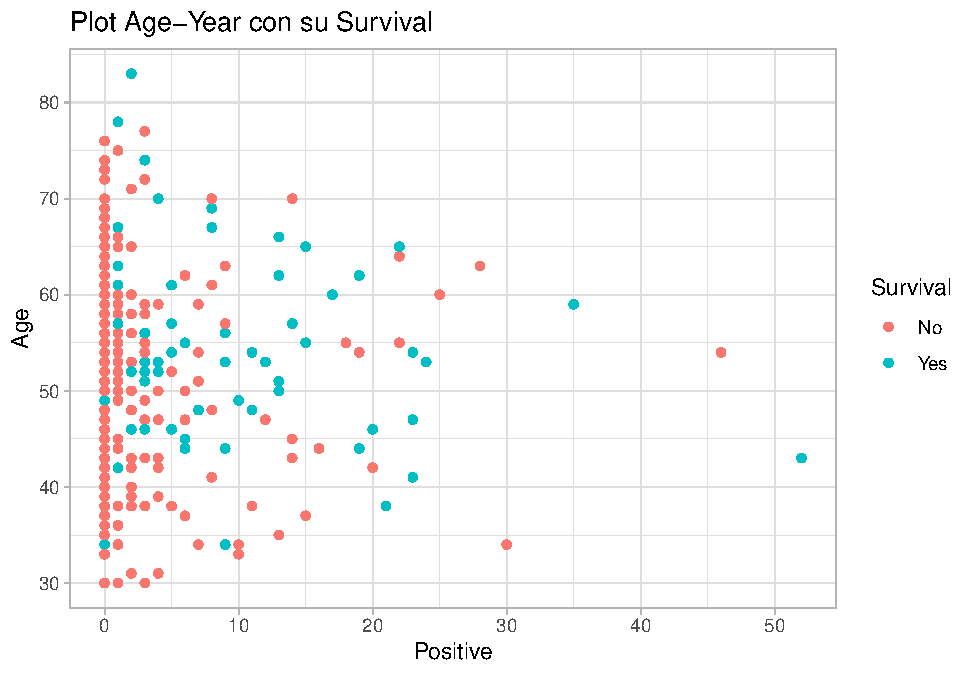
\includegraphics[width=.9\linewidth]{img/Clasificacion_files/figure-latex/unnamed-chunk-5-2}\caption{}\end{figure}

\begin{figure}[H]\center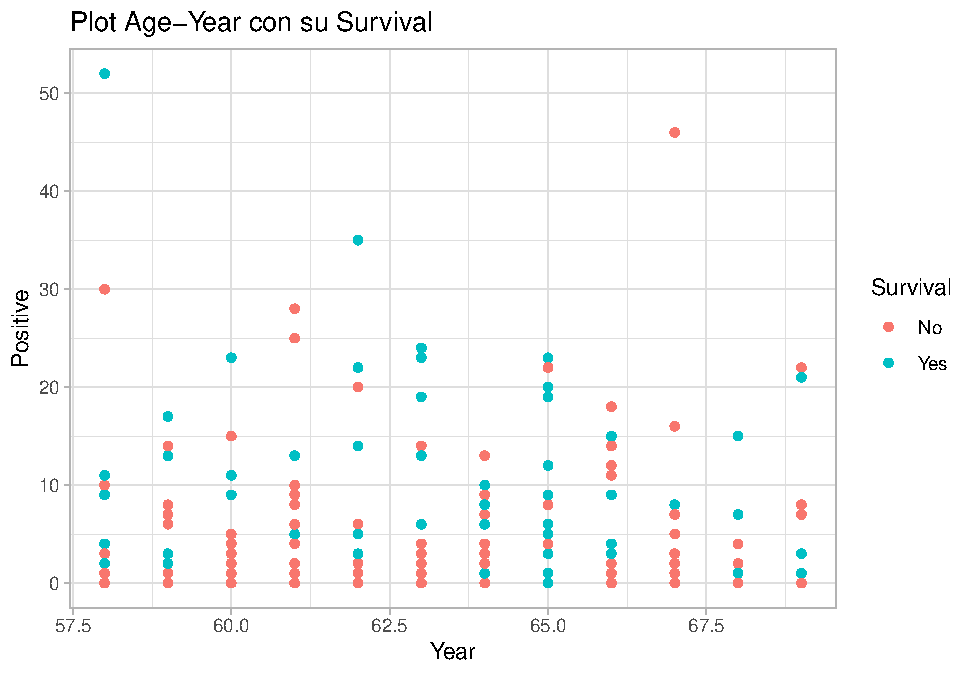
\includegraphics[width=.9\linewidth]{img/Clasificacion_files/figure-latex/unnamed-chunk-5-3}\caption{}\end{figure}

\begin{figure}[H]\center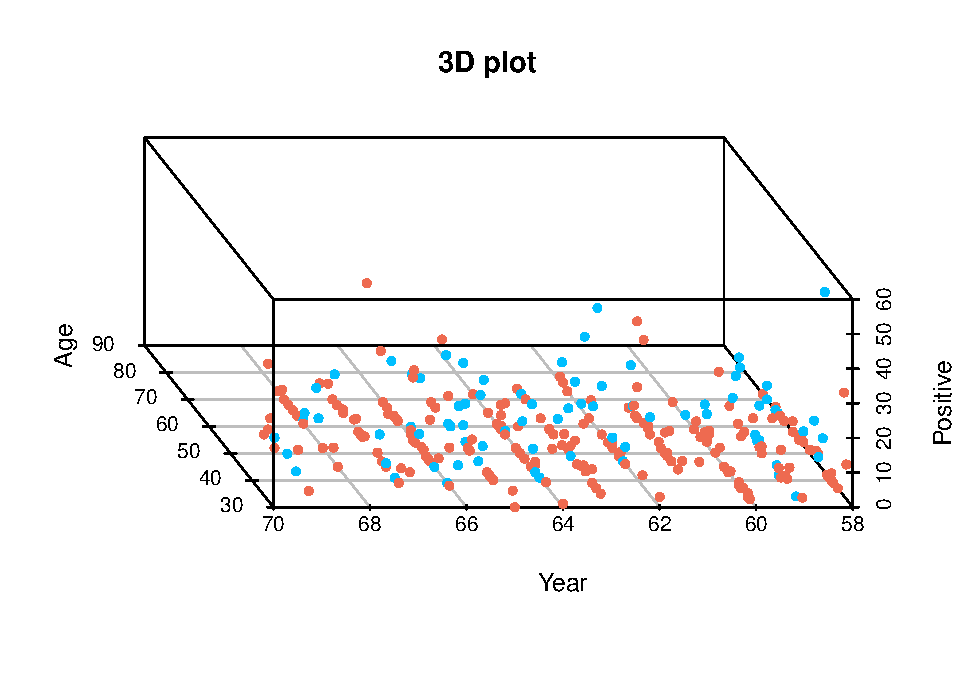
\includegraphics[width=.9\linewidth]{img/Clasificacion_files/figure-latex/unnamed-chunk-6-1}\caption{}\end{figure}

\begin{figure}[H]\center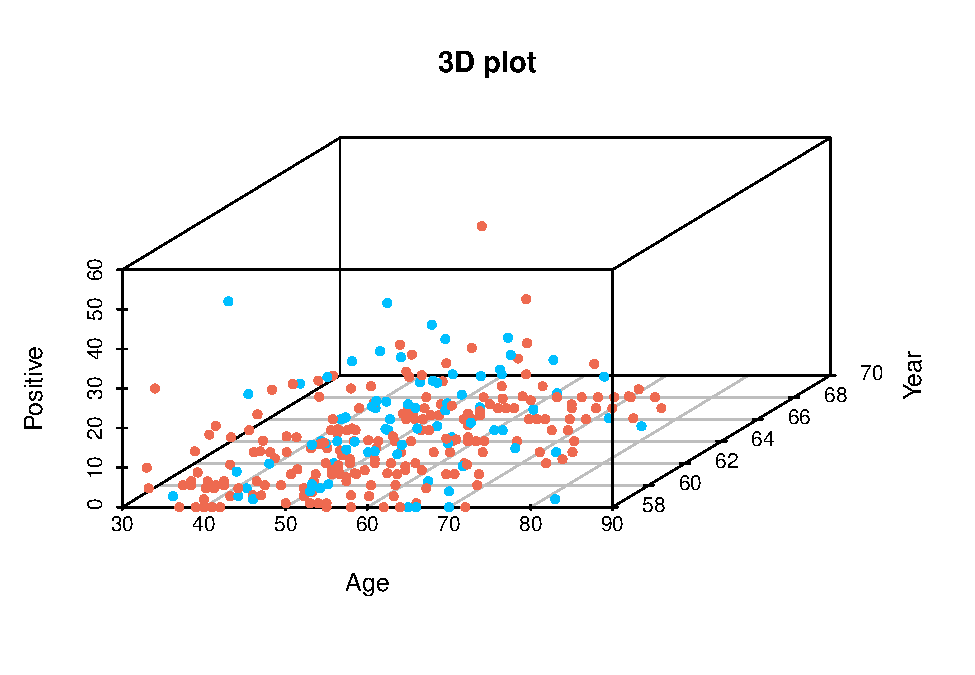
\includegraphics[width=.9\linewidth]{img/Clasificacion_files/figure-latex/unnamed-chunk-6-2}\caption{}\end{figure}

De cara a un algoritmo KNN, apreciamos los datos muy entremezclados, con mayor tendencia a agruparse los no supervivientes que los que sí, pero nada en especial que nos llame la atención.

\vspace{\baselineskip}

Debido a esto vamos a empezar con un valor de K relativamente bajo y vamos a ir aumentándolo poco a poco. Tenemos que tener en cuenta que un K mayor puede ocasionar overfitting, pero usando técnicas de cross-validation podemos minimizar las posibilidades.

Los resultados usando el paquete caret son los siguientes\footnote{Los datos han sido preprocesados con una estandarización antes de aplicar cualquiera de los algoritmos}:
\begin{verbatim}
k-Nearest Neighbors 

275 samples
  3 predictor
  2 classes: 'No', 'Yes' 

No pre-processing
Resampling: Cross-Validated (10 fold) 
Summary of sample sizes: 248, 247, 247, 247, 247, 247, ... 
Resampling results across tuning parameters:

  k   Accuracy   Kappa    
   3  0.6947599  0.2034939
   4  0.6832418  0.1615034
   5  0.6884412  0.1100164
   6  0.6879121  0.1426382
   7  0.6950549  0.0983539
   8  0.7165954  0.1496547
   9  0.7240130  0.1881672
  10  0.7164632  0.1470534
  11  0.7277269  0.1753847
  12  0.7203195  0.1708068
  13  0.7241656  0.1767408
  14  0.7313085  0.2015352
  15  0.7422873  0.2320214

Accuracy was used to select the optimal model using the largest value.
The final value used for the model was k = 15.
\end{verbatim}

Vemos que al estar los datos tan entremezclados ni siquiera con un K pequeño aprende bien, es ya con un K medianamente alto (= 15) donde obtiene mayor accuracy en training.

Una vez más probablemente esto se deba a la gran mezcla de los datos, de forma que necesite la ``opinión'' de un gran número de vecinos para poder predecir con mayor confianza el nuevo valor.

\begin{figure}[H]\center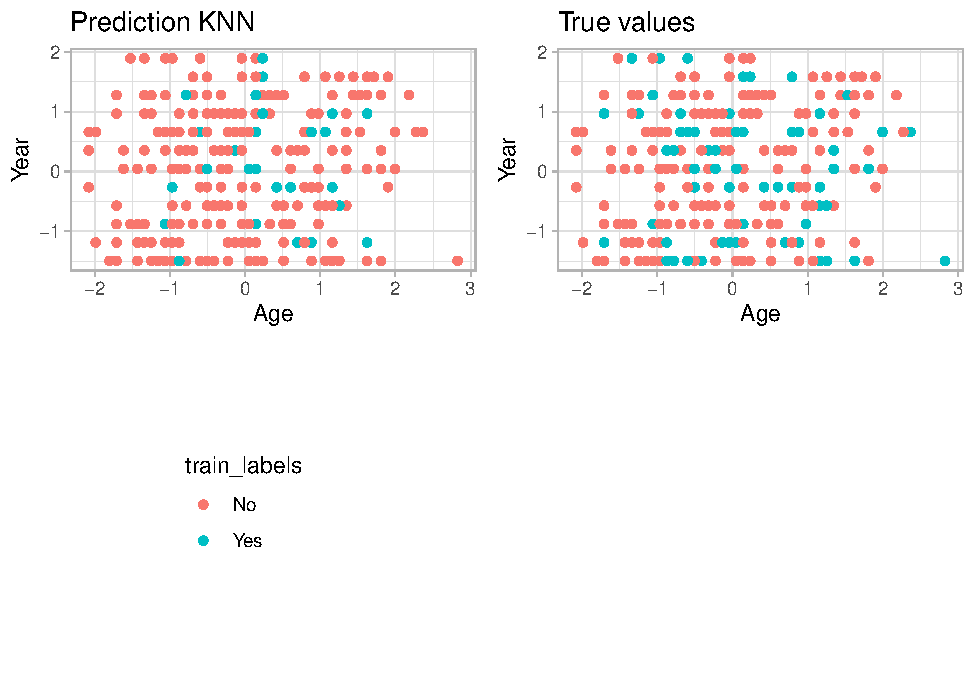
\includegraphics[width=.9\linewidth]{img/Clasificacion_files/figure-latex/unnamed-chunk-10-1}\caption{Predicción con K=15 en training}\end{figure}

Vemos que el uso de un K alto hace que perdamos puntos de Yes. Probablemente al ser minoría el error cometido clasificándolos como No es menor y por eso obtiene mejor accuracy.

\vspace{\baselineskip}

Una evaluación con el subconjunto reservado inicialmente como test nos muestra una calidad extrañamente superior que la de training.

\begin{verbatim}
Test evaluation:
 Accuracy     Kappa 
0.9032258 0.5181347 

Confusion matrix (in test split):
knnPred No Yes
    No  26   2
    Yes  1   2
\end{verbatim}

\begin{figure}[H]\center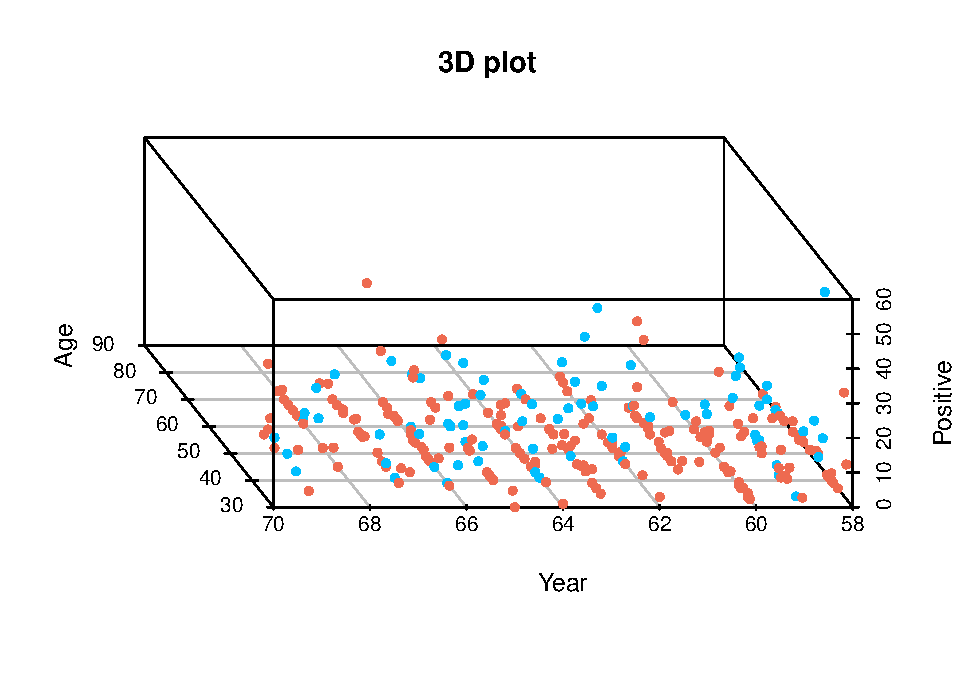
\includegraphics[width=.9\linewidth]{img/Clasificacion_files/figure-latex/unnamed-chunk-9-1}\caption{Matriz de confusión sobre el conjunto de test}\end{figure}

Este comportamiento no es el habitual en aprendizaje automático, parece que casualmente el conjunto de test es bastante fácil de ajustar y por eso se obtienen mejores resultados que en training.
En la sección ?? se muestran las etiquetas. También se vuelve a incidir en la alta presencia de etiquetas \textit{No}.

El valor alto de K hace que se prediga con mayor facilidad este valor de etiqueta y por ese desbalanceo se obtengan tan buenos resultados. En sí es un poco preocupante de cara a la población real de los datos, pero debemos suponer que la muestra que tenemos es representativa y por tanto válida.

Por otro lado, para el problema que nos atañe quizás esto podría ser incluso un hecho positivo, ya que los falsos positivos sería algo que querríamos evitar a toda costa.

\vspace{\baselineskip}

Por comparar, podemos también evaluar con otros valores de K en test. Puesto que hemos obtenido los mejores resultados en training con un K de 15, que es un valor relativamente alto, podemos probar con uno bajo y uno intermedio (3 y 7).

\begin{verbatim}
k-Nearest Neighbors

No pre-processing
Resampling: Cross-Validated (10 fold) 
Summary of sample sizes: 248, 247, 248, 248, 247, 247, ... 
Resampling results:

  Accuracy  Kappa    
  0.697619  0.1988554

Tuning parameter 'k' was held constant at a value of 3
\end{verbatim}

\begin{verbatim}
Test evaluation:
Accuracy     Kappa 
0.8064516 0.1388889

Confusion matrix (in test split):
         test_labels
knn3Pred   No Yes
     No    24   3
     Yes    3   1
\end{verbatim}

\begin{figure}[H]\center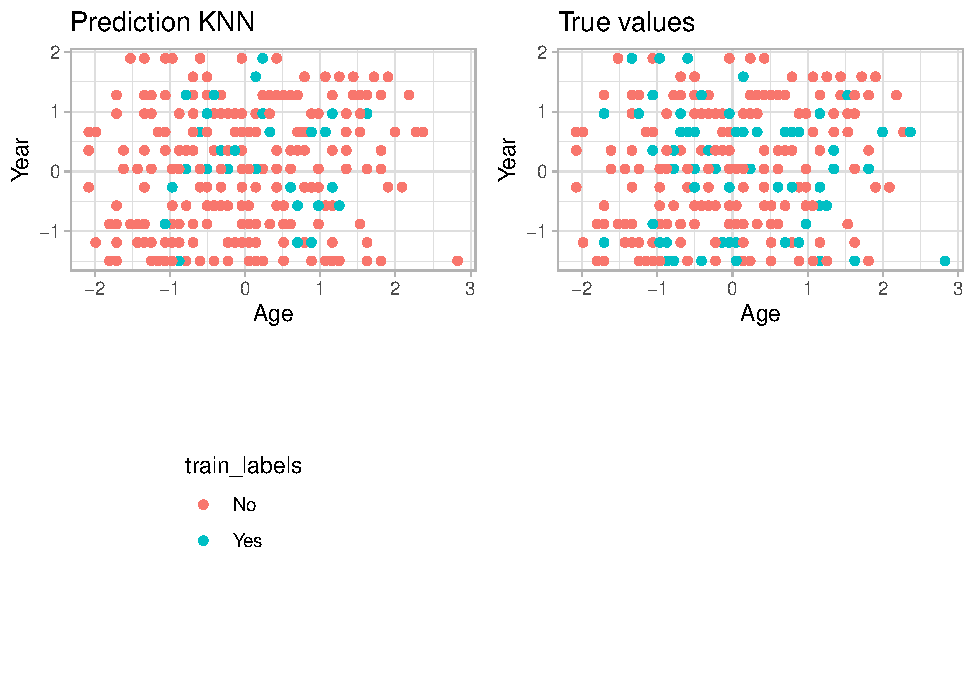
\includegraphics[width=.9\linewidth]{img/Clasificacion_files/figure-latex/unnamed-chunk-12-1}\caption{Matriz de confusión sobre el conjunto de test}\end{figure}

\newpage

\begin{verbatim}
k-Nearest Neighbors 

No pre-processing
Resampling: Cross-Validated (10 fold) 
Summary of sample sizes: 248, 247, 247, 248, 248, 247, ... 
Resampling results:

  Accuracy   Kappa     
  0.6761905  0.08141897

Tuning parameter 'k' was held constant at a value of 7
\end{verbatim}

\begin{verbatim}
Test evaluation:
Accuracy     Kappa 
0.8064516 0.1388889

Confusion matrix (in test split):
        test_labels
knn7Pred No Yes
     No  24   3
     Yes  3   1 
\end{verbatim}

\begin{figure}[H]\center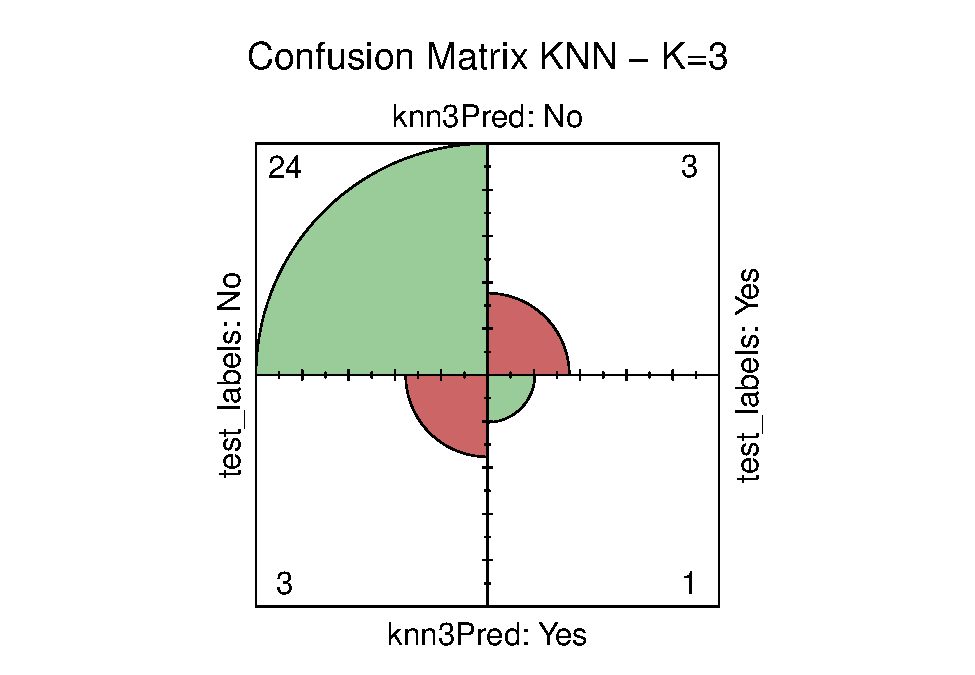
\includegraphics[width=.9\linewidth]{img/Clasificacion_files/figure-latex/unnamed-chunk-14-1}\caption{Matriz de confusión sobre el conjunto de test}\end{figure}

K=7 vemos que es el que más sufre al evaluar en test, y ambos (tal y como nos había indicado la primera ejecución con CV) tienen una calidad bastante inferior (tanto en training como en test) a un K=15.

\subsection{Algoritmo LDA}
\subsubsection{Asunciones}
Comprobamos asunciones:
\begin{enumerate}
    \item \textbf{Distribución aleatoria}: No nos queda más remedio que creer que sí.
    \item \textbf{Cada predictor sigue una distribución normal}: Ya vimos en el EDA que esto no era cierto. El test de Shapiro nos aseguraba que no había normalidad y los QQ-plots nos lo hacían ver claramente. Técnicamente sabiendo esto no deberíamos usar LDA, pero puesto que esto es un proyecto seguimos.
    
    Por otro lado, las variables Age y Year no parecen seguir una distribución demasiado ``rara'' (en comparación con una normal), por lo que es posible que obtengamos resultados de calidad aceptable.
    \item \textbf{Las clases siguen la misma matriz de covarianza}: Lo comprobamos a continuación.
\end{enumerate}

Calculamos la diagonal de la matriz de correlación para cada una de las clases, obteniendo:
\begin{verbatim}
Para clase Yes:
      Age      Year  Positive 
0.9176155 1.0113109 1.6788033 

Para clase No:
      Age      Year  Positive 
1.0756415 0.9752581 0.5448553 
\end{verbatim}

\vspace{\baselineskip}

Estos valores nos parecen indicar que las variables Age y Positive parecen seguir distintas varianzas, pero es preferible asegurarlo con un test estadístico.

Puesto que nuestras variables no siguen una distribución normal, no podemos hacer el test de homogeneidad de Barlett. Utilizamos por tanto el de Levene
\begin{verbatim}
Age:
\end{verbatim}

\begin{tabular}{l|r|r|r}
\hline
  & Df & F value & Pr(>F)\\
\hline
group & 1 & 1.799898 & 0.1807261\\
\hline
 & 304 &  & \\
\hline
\end{tabular}

\begin{verbatim}
Year:
\end{verbatim}

\begin{tabular}{l|r|r|r}
\hline
  & Df & F value & Pr(>F)\\
\hline
group & 1 & 0.0624405 & 0.8028481\\
\hline
 & 304 &  & \\
\hline
\end{tabular}

\begin{verbatim}
Positive:
\end{verbatim}

\begin{tabular}{l|r|r|r}
\hline
  & Df & F value & Pr(>F)\\
\hline
group & 1 & 18.78912 & 1.99e-05\\
\hline
 & 304 &  & \\
\hline
\end{tabular}

Indicándonos que solo se puede asegurar que la variable Positive no tiene homogeneidad entre clases diferentes.

\vspace{\baselineskip}

Gráficamente:

\begin{figure}[H]\center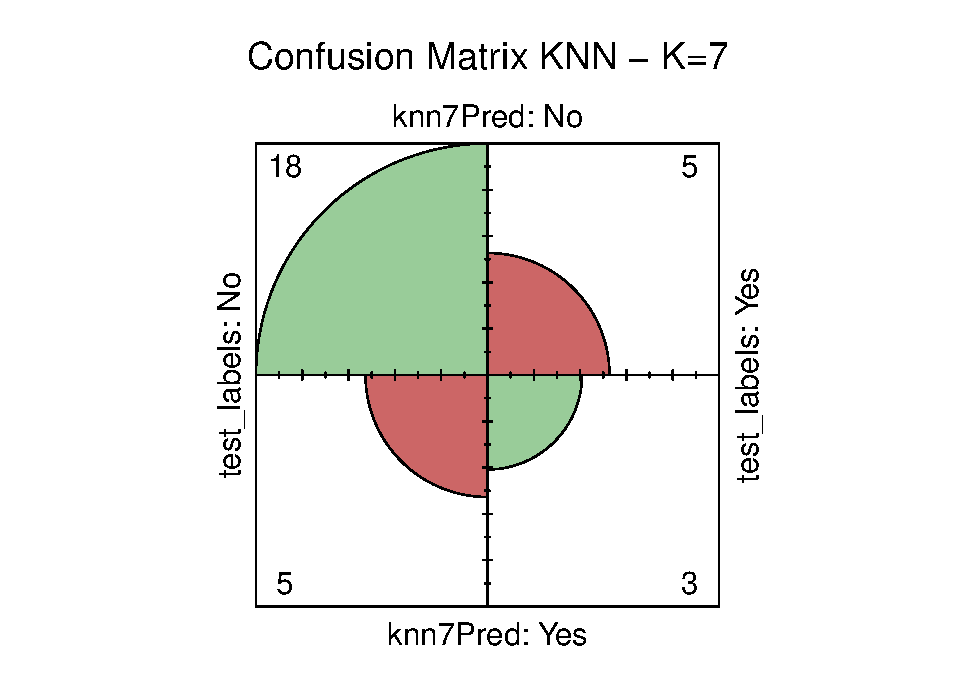
\includegraphics[width=.8\linewidth]{img/Clasificacion_files/figure-latex/unnamed-chunk-17-1}\caption{}\end{figure}

\begin{figure}[H]\center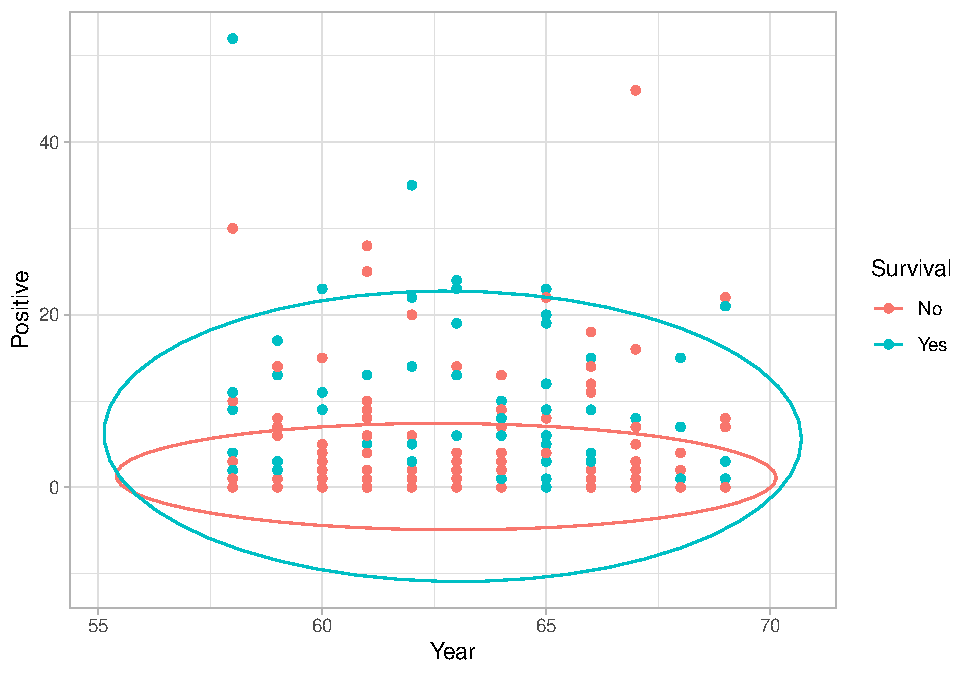
\includegraphics[width=.8\linewidth]{img/Clasificacion_files/figure-latex/unnamed-chunk-17-2}\caption{}\end{figure}

\begin{figure}[H]\center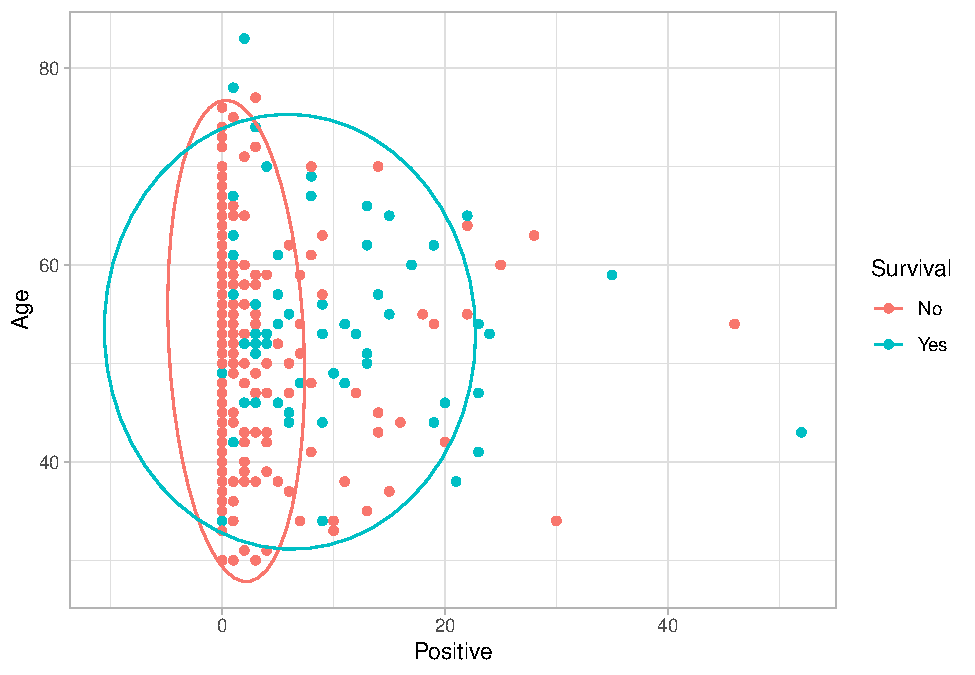
\includegraphics[width=.8\linewidth]{img/Clasificacion_files/figure-latex/unnamed-chunk-17-3}\caption{}\end{figure}

\begin{figure}[H]\center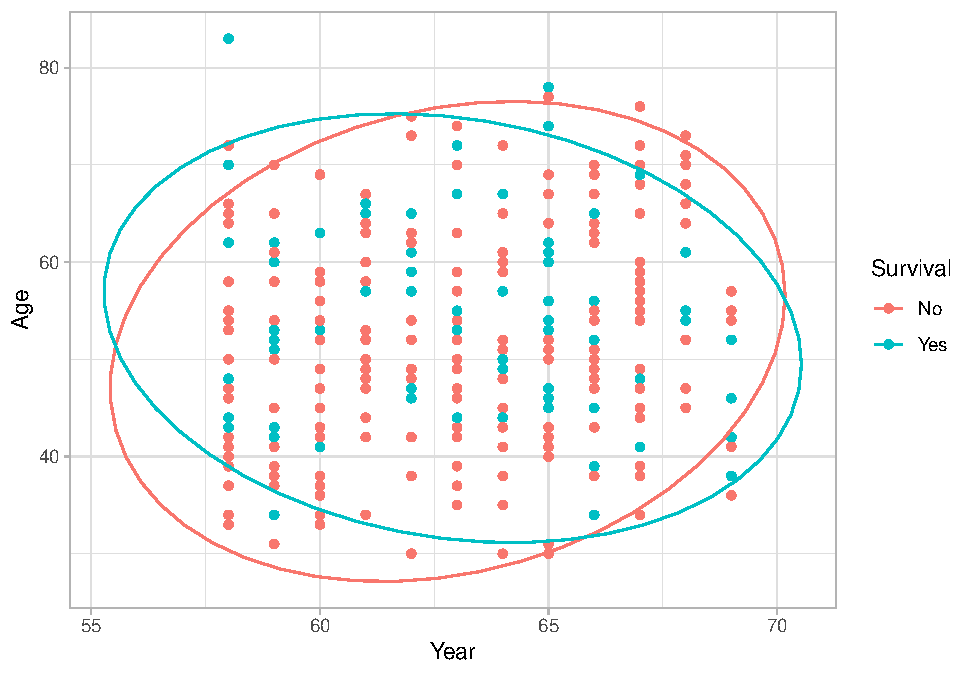
\includegraphics[width=.8\linewidth]{img/Clasificacion_files/figure-latex/unnamed-chunk-18-1}\caption{}\end{figure}

\begin{figure}[H]\center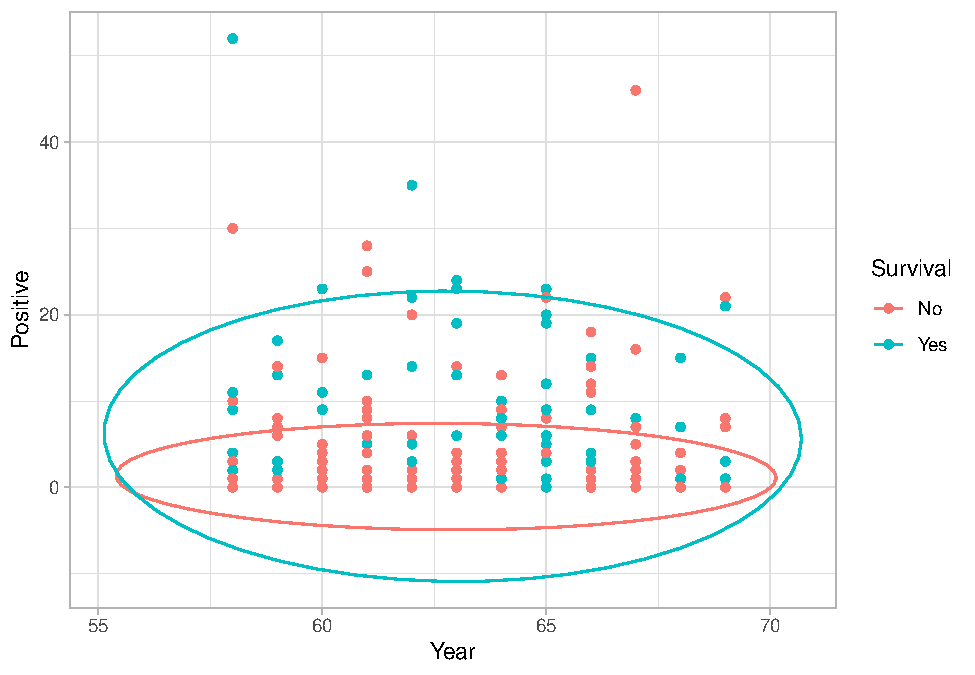
\includegraphics[width=.8\linewidth]{img/Clasificacion_files/figure-latex/unnamed-chunk-18-2}\caption{}\end{figure}

\begin{figure}[H]\center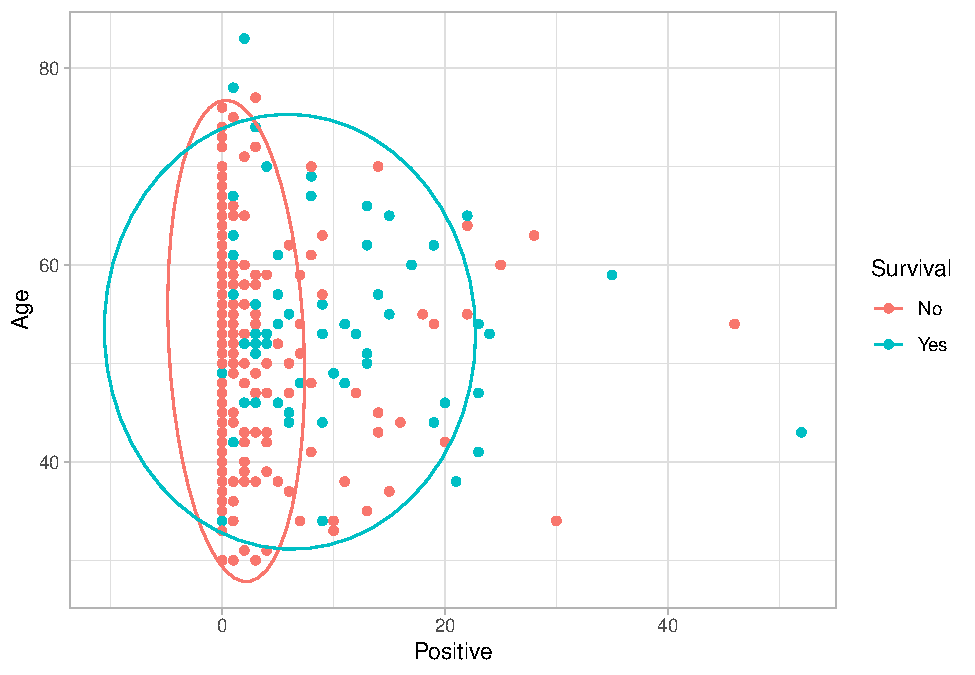
\includegraphics[width=.8\linewidth]{img/Clasificacion_files/figure-latex/unnamed-chunk-18-3}\caption{}\end{figure}

Se nota que la causa de que no se rechace el test para esta variable es la gran cantidad de datos con Positive igual a 0.

\vspace{\baselineskip}

Por tanto para LDA no podemos hacer uso de la variable Positive, puesto que además de la falta de normalidad se incumpliría la asunción número 3, por lo que usamos las otras dos.

\vspace{\baselineskip}

Aunque solo es recomendable, y no son cualidades necesarias para obtener solución en LDA:
\begin{itemize}
    \item Tenemos más instancias que predictores, por varios órdenes de magnitud.
    \item Los predictores son independientes. 
    \item No tenemos varianza cercana a cero.
\end{itemize}

\subsubsection{Aplicación del algoritmo LDA}

\begin{verbatim}
Call:
lda(x, y)

Prior probabilities of groups:
  No  Yes 
0.72 0.28 

Group means:
            Age        Year
No  -0.04141411 0.004845716
Yes  0.11031976 0.021276742

Coefficients of linear discriminants:
            LD1
Age  0.98140853
Year 0.03411981
Cross-Validated (10 fold) Confusion matrix (in test split) 

(entries are percentual average cell counts across resamples)
 
          Reference
Prediction No Yes
       No  72  28
       Yes  0   0
                          
 Accuracy (average) : 0.72
\end{verbatim}

\begin{figure}[H]\center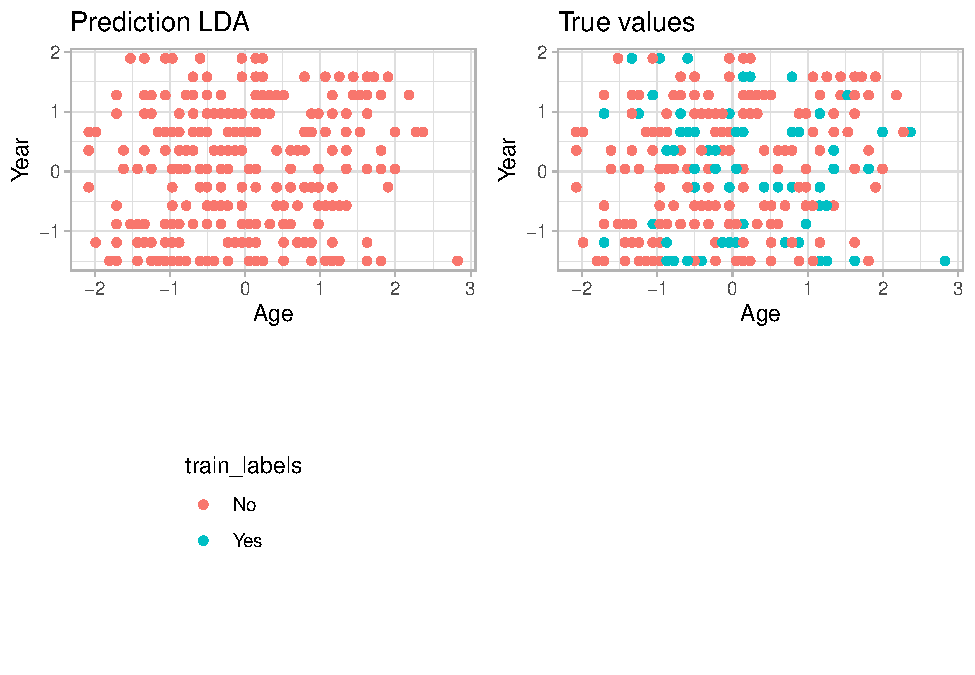
\includegraphics[width=.9\linewidth]{img/Clasificacion_files/figure-latex/unnamed-chunk-22-1}\caption{Predicciones LDA sobre training}\end{figure}

Hacemos un plot del ajuste

\begin{figure}[H]\center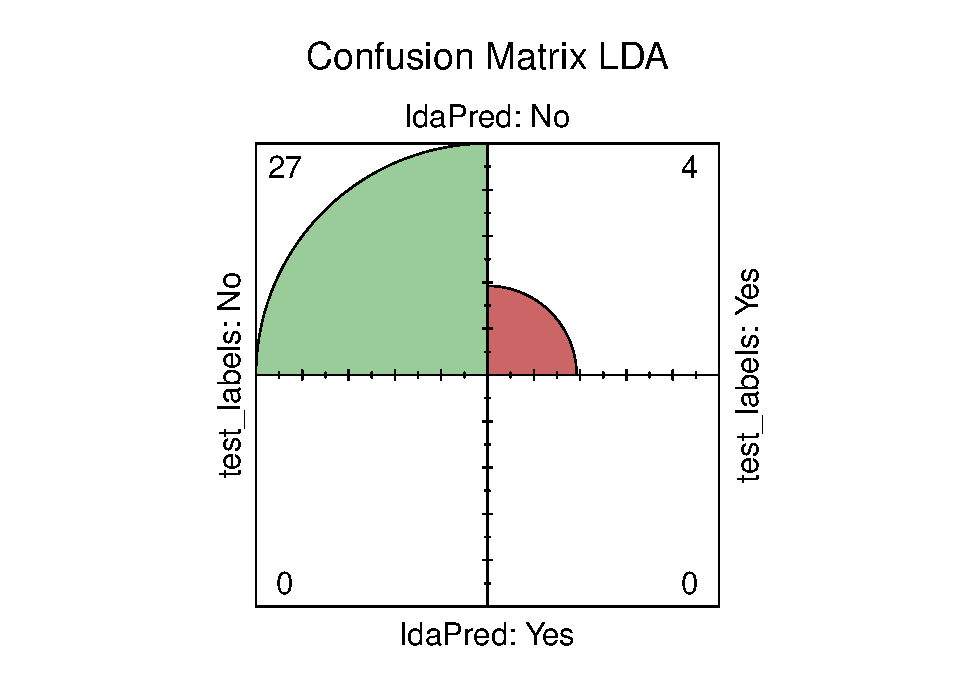
\includegraphics[width=.9\linewidth]{img/Clasificacion_files/figure-latex/unnamed-chunk-23-1}\caption{}\end{figure}

\begin{figure}[H]\center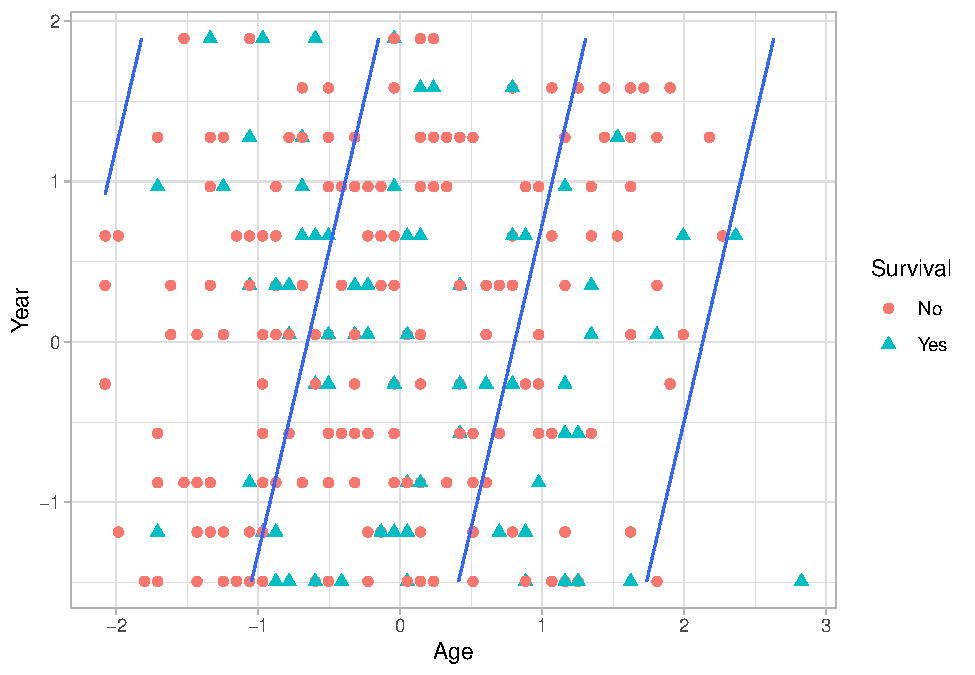
\includegraphics[width=.9\linewidth]{img/Clasificacion_files/figure-latex/unnamed-chunk-24-1}\caption{}\small{Estamos pintando un contorno 3D y por eso nos salen múltiples líneas en el gráfico}\end{figure}

Predecimos en test

\begin{verbatim}
Test evaluation:
Accuracy     Kappa 
0.8709677 0.0000000 

Confusion matrix (in test split):
       test_labels
ldaPred No Yes
    No  27   4
    Yes  0   0
\end{verbatim}

\begin{figure}[H]\center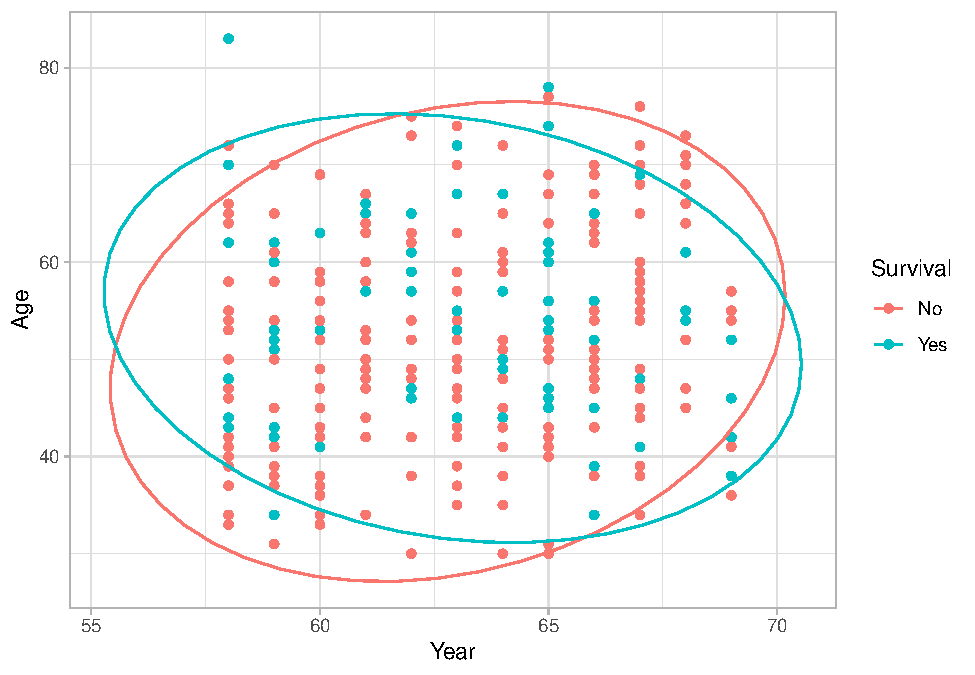
\includegraphics[width=.9\linewidth]{img/Clasificacion_files/figure-latex/unnamed-chunk-21-1}\caption{Matriz de confusión sobre el conjunto de test}\end{figure}

Tenemos un dataset bastante desbalanceado, y LDA no predice para la clase Yes. Con esto se asegura un alto accuracy en nuestro entrenamiento, pero no asegura de que para datos externos vaya a ser así. Pese a ello, no nos queda más remedio que suponer que nuestros datos vienen de la misma muestra aleatoria y por tanto son releventes para la clasificación.

\subsection{Algoritmo QDA}
\subsubsection{Asunciones}

QDA tiene las mismas asunciones de LDA salvo que relaja la norma de que las clases tengan igual covarianza. Esto nos permite usar la variable Positive que habíamos descartado en LDA.

\vspace{\baselineskip}

Por tanto tenemos los requisitos de: 
\begin{enumerate}
    \item Distribución aleatoria.
    \item Distribución normal.
\end{enumerate}

Técnicamente el no cumplir normalidad no imposibilita que se encuentre solución, pero ya no nos lo asegura.

\vspace{\baselineskip}

Adicionalmente tenemos de forma recomendada que: 
\begin{itemize}
    \item El número de predictores debe ser menor que el número de instancias de cada clase. 
    
    Del EDA sabemos que esto es cierto.
    \item Los predictores dentro de cada clase no deben estar correlacionados.
    
    Esto podemos verlo mediante matrices de correlación.
\end{itemize}

\begin{figure}[H]\center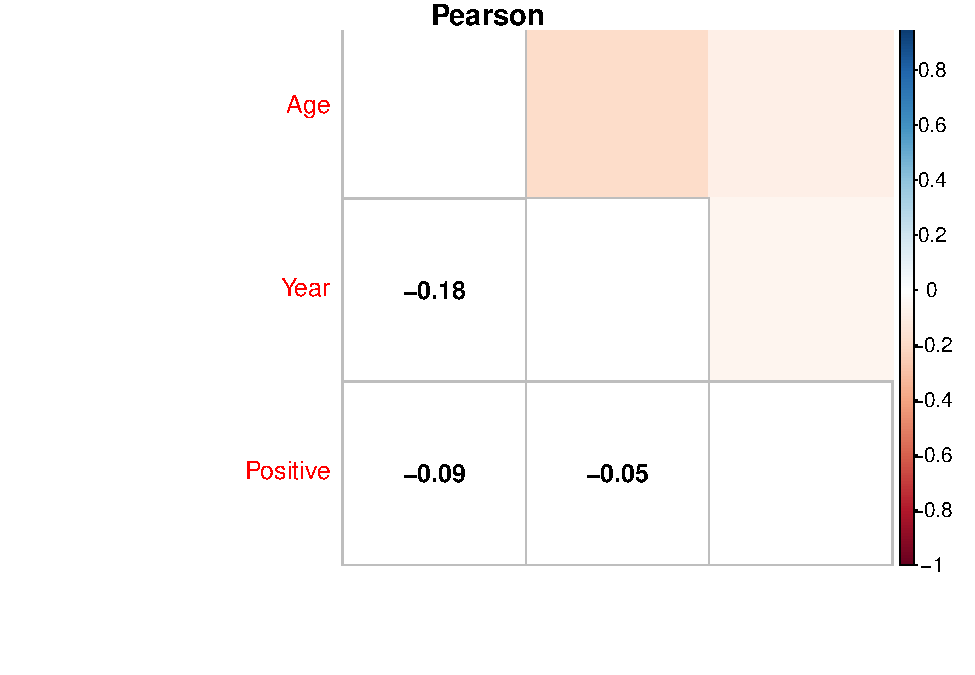
\includegraphics[width=.9\linewidth]{img/Clasificacion_files/figure-latex/unnamed-chunk-25-1}\caption{Matriz de correlación para la clase \textit{Yes}}\end{figure}

\begin{figure}[H]\center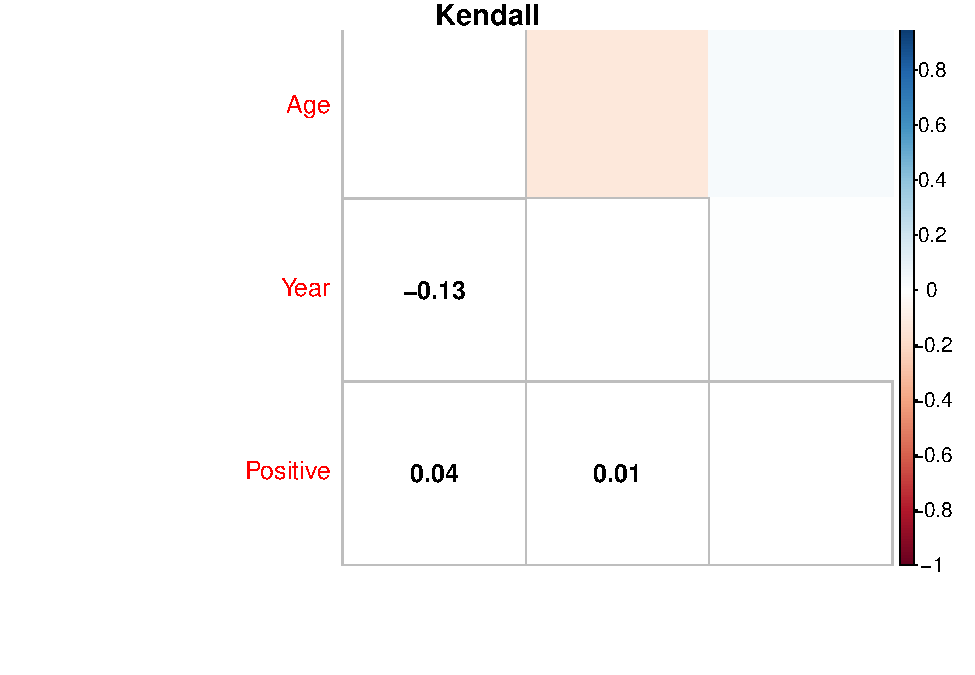
\includegraphics[width=.9\linewidth]{img/Clasificacion_files/figure-latex/unnamed-chunk-25-2}\caption{Matriz de correlación para la clase \textit{Yes}}\end{figure}

\begin{figure}[H]\center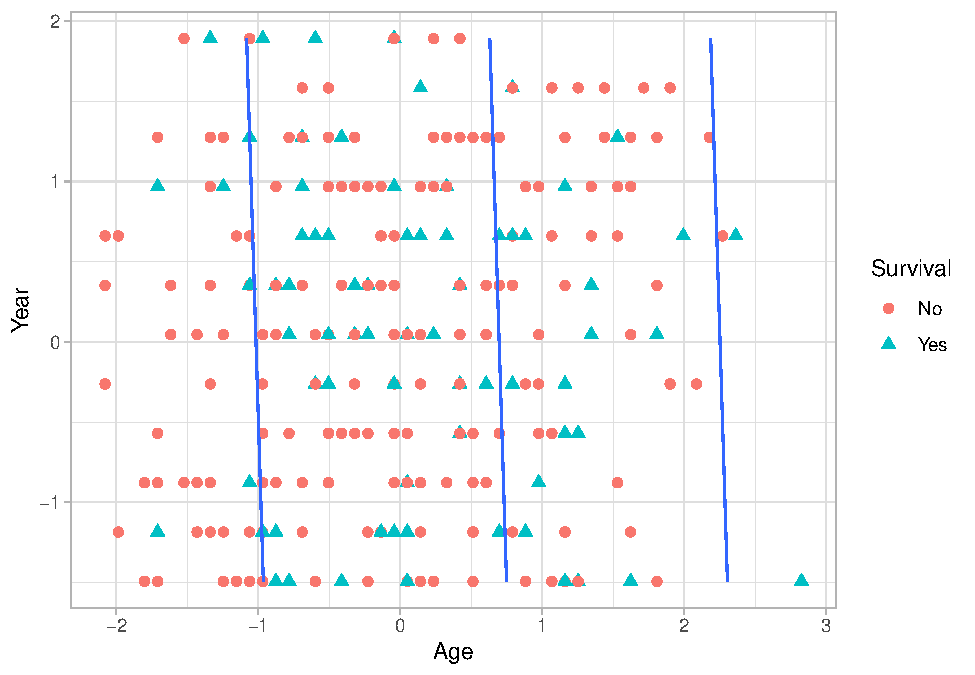
\includegraphics[width=.9\linewidth]{img/Clasificacion_files/figure-latex/unnamed-chunk-26-1}\caption{Matriz de correlación para la clase \textit{No}}\end{figure}

\begin{figure}[H]\center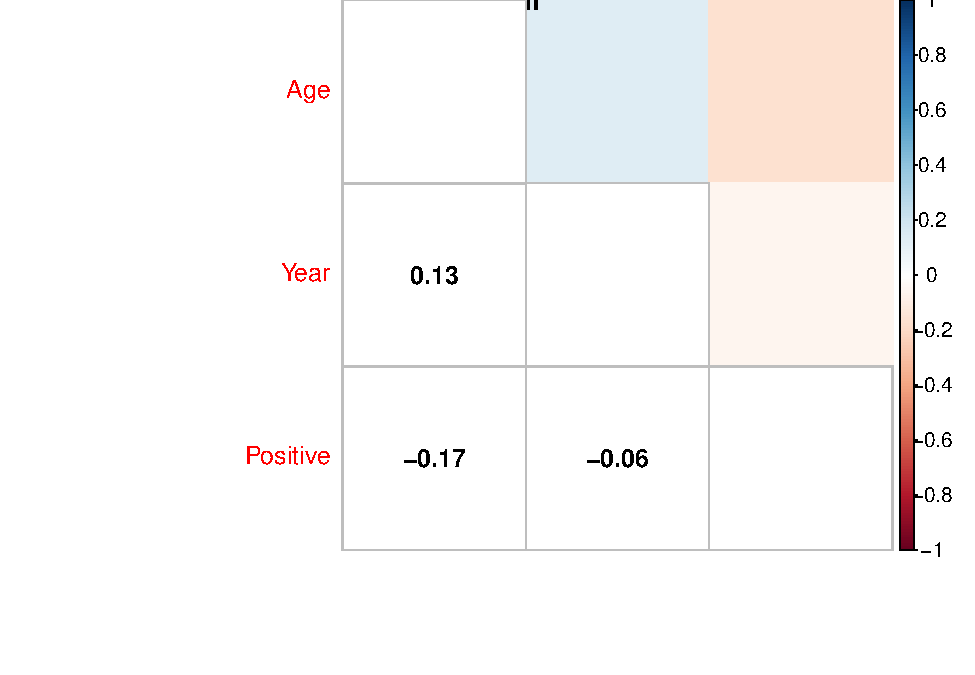
\includegraphics[width=.9\linewidth]{img/Clasificacion_files/figure-latex/unnamed-chunk-26-2}\caption{Matriz de correlación para la clase \textit{Yes}}\end{figure}

\subsubsection{Aplicación del algoritmo QDA}

\begin{verbatim}
Call:
qda(x, y)

Prior probabilities of groups:
  No  Yes 
0.72 0.28 

Group means:
            Age        Year   Positive
No  -0.04141411 0.004845716 -0.1792534
Yes  0.11031976 0.021276742  0.4804648
Cross-Validated (10 fold) Confusion matrix (in test split) 

(entries are percentual average cell counts across resamples)
 
          Reference
Prediction   No  Yes
       No  67.3 21.5
       Yes  4.7  6.5
                            
 Accuracy (average) : 0.7382
\end{verbatim}

\begin{figure}[H]\center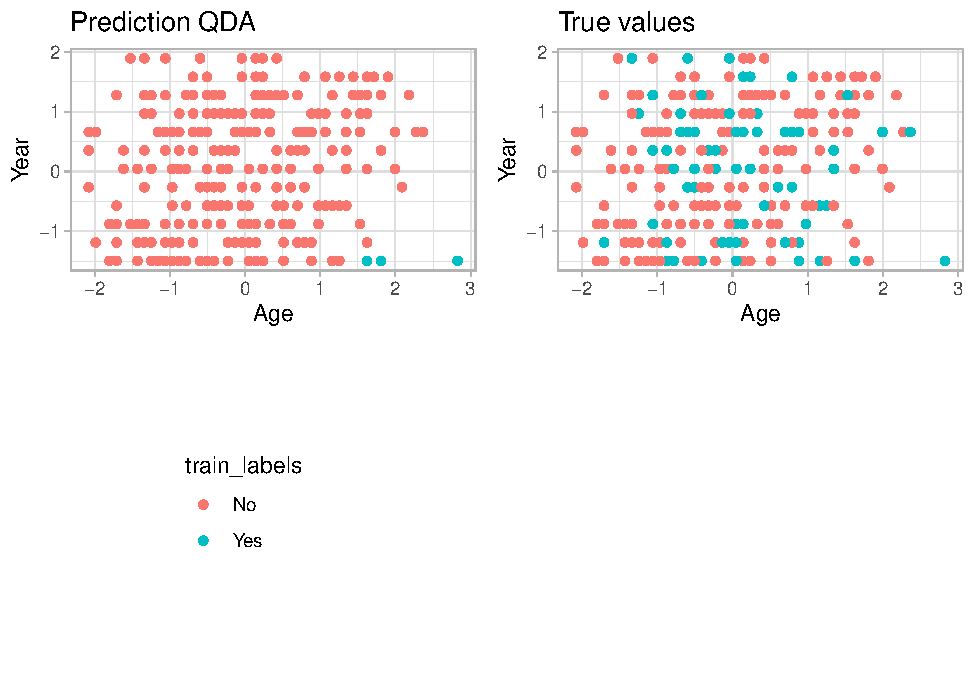
\includegraphics[width=.9\linewidth]{img/Clasificacion_files/figure-latex/unnamed-chunk-30-1}\caption{Predicciones QDA sobre training}\end{figure}


\begin{verbatim}
Test evaluation:
Accuracy     Kappa 
0.8709677 0.2705882

Confusion matrix (in test split):
       test_labels
qdaPred No Yes
    No  26   3
    Yes  1   1
\end{verbatim}

\begin{figure}[H]\center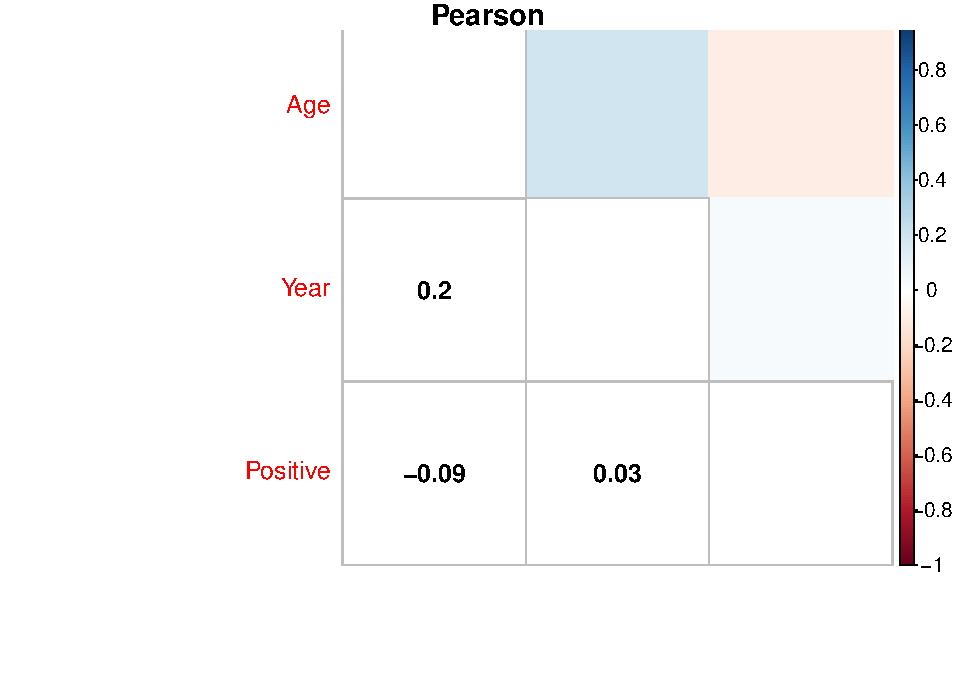
\includegraphics[width=.9\linewidth]{img/Clasificacion_files/figure-latex/unnamed-chunk-29-1}\caption{Matriz de confusión sobre el conjunto de test}\end{figure}

Obtenemos la mismos accuracy que LDA, pero en este caso vemos que sí se predice la clase Yes.

\subsection{Comparativa de algoritmos}
\subsubsection{Para el dataset \textit{haberman}}

Si nos fijamos únicamente en los resultados obtenidos para este problema, los tres algoritmos obtienen el mismo accuracy en nuestro conjunto de test\footnote{Puesto que hemos usado el paquete caret, no podemos comparar con los datos de accuracy que nos proporciona su salida. Los datos aquí mostrados hacen referencia a una evaluación de los modelos devueltos sobre el conjunto inicialmente reservado de test.}. Aunque las etiquetas de este conjunto contienen elementos de ambas clases, podemos ver que se predice mayoritariamente la clase \textit{No}. Como se había mencionado nuestro dataset está bastante desbalanceado, por lo que era más probable que se predijera esa clase con mayor facilidad.

\begin{verbatim}
Etiquetas:
No  No  Yes No  No  No  No  No  Yes No  No  No  No  No  No  No  No  Yes No 
No  No  No  No  No  No  No  No  Yes No  No  No 

Predicciones KNN:
No  No  Yes No  No  No  No  Yes No  No  No  No  No  No  No  No  No  Yes No 
No  No  No  No  No  No  No  No  No  No  No  No 

Predicciones LDA:
No No No No No No No No No No No No No No No No No No No No No No No No No
No No No No No No

Predicciones QDA:
No  No  Yes No  No  No  No  Yes No  No  No  No  No  No  No  No  No  No  No 
No  No  No  No  No  No  No  No  No  No  No  No 
\end{verbatim}

\vspace{\baselineskip}

\begin{verbatim}
Accuracy KNN:
 Accuracy     Kappa 
0.9032258 0.5181347 

Accuracy LDA:
 Accuracy     Kappa 
0.8709677 0.0000000 

Accuracy QDA:
 Accuracy     Kappa 
0.8709677 0.2705882 
\end{verbatim}

\begin{figure}[H]\center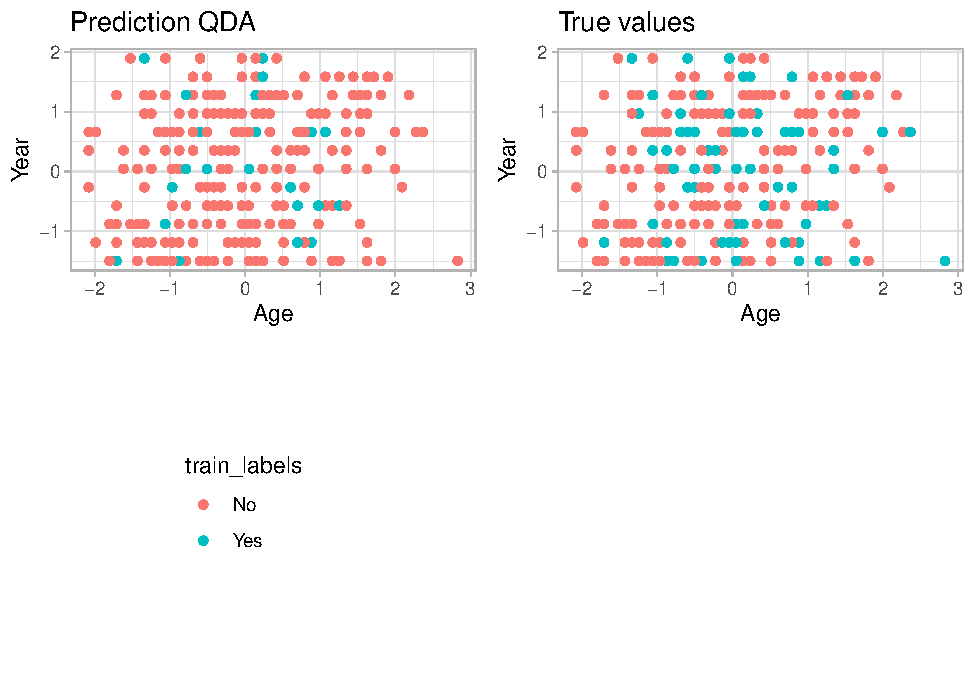
\includegraphics[width=.9\linewidth]{img/Clasificacion_files/figure-latex/unnamed-chunk-33-1}\caption{}\end{figure}

Obtenemos valores de accuracy muy similares, pero diferentes valores de Kappa, siendo en general todos bajos.

\vspace{\baselineskip}

Pese a esto, y ya no solo por tener mejores resultados, sino por no cumplir las asunciones necesarias de obtener resultados de calidad en LDA y QDA, para este problema optaríamos por usar el algoritmo KNN.

A partir de las gráficas 3D de las figuras ?? y ?? se apreció una difícil separación de las clases, por lo que el algoritmo de vecinos más cercanos nos resulta una aproximación más lógica.

\subsubsection{Comparativas generales}

Para comparar la calidad genérica de los algoritmos vamos a aplicar test estadísticos en base a los resultados obtenidos en múltiples datasets.

\vspace{\baselineskip}

Estas son las tablas de resultados que tenemos para test:

\begin{tabular}{l|r|r|r}
\hline
Dataset & out\_test\_knn & out\_test\_lda & out\_test\_qda\\
\hline
appendicitis & 0.8966667 & 0.8690909 & 0.8109091\\
\hline
australian & 0.6838235 & 0.8579710 & 0.8028986\\
\hline
balance & 0.9024546 & 0.8624101 & 0.9167905\\
\hline
bupa & 0.6865775 & 0.6837924 & 0.5991759\\
\hline
contraceptive & 0.5448653 & 0.5091561 & 0.5173102\\
\hline
haberman & 0.7462069 & 0.7481720 & 0.7512903\\
\hline
hayes-roth & 0.5666667 & 0.5500000 & 0.5875000\\
\hline
heart & 0.6692308 & 0.8481481 & 0.8296296\\
\hline
iris & 0.9642857 & 0.9800000 & 0.9733333\\
\hline
led7digit & 0.7510204 & 0.7420000 & 0.6975000\\
\hline
mammographic & 0.7977698 & 0.8241269 & 0.8194042\\
\hline
monk-2 & 0.9743632 & 0.7703433 & 0.9235535\\
\hline
newthyroid & 0.9071429 & 0.9164502 & 0.9629870\\
\hline
pima & 0.7348861 & 0.7709930 & 0.7412403\\
\hline
tae & 0.3838095 & 0.5245833 & 0.5425000\\
\hline
titanic & 0.7850353 & 0.7760304 & 0.7733032\\
\hline
vehicle & 0.6291452 & 0.7813305 & 0.8522409\\
\hline
vowel & 0.6428571 & 0.6030303 & 0.9191919\\
\hline
wine & 0.6959559 & 0.9944444 & 0.9888889\\
\hline
wisconsin & 0.9735023 & 0.9592185 & 0.9519476\\
\hline
\end{tabular}

\vspace{\baselineskip}

Aplicamos el test de Wilcoxon a cada pareja de algoritmos:

\vspace{\baselineskip}

\textbf{LDA vs QDA:} Obtenemos un ranking de 144 para LDA y 96 para QDA, con un p-valor de 0.75 (o nivel de confianza del 25\%).
\begin{verbatim}
V = 96, p-value = 0.7562
alternative hypothesis: true location shift is not equal to 0

  V    V
114 - 96 
\end{verbatim}

Esto nos dice que LDA obtiene mejores resultados pero puesto que el p-value es extremadamente grande no podemos afirmar con garantía estadística que las diferencias entre los tests sean notorias.

\vspace{\baselineskip}

\textbf{LDA vs KNN:} Ahora obtenemos un ranking de 90 para LDA y 120 para QDA, con un p-valor de 0.59 (o nivel de confianza del 41\%).
\begin{verbatim}
V = 120, p-value = 0.5958
alternative hypothesis: true location shift is not equal to 0

 V     V
90 - 120 
\end{verbatim}

Seguimos teniendo un p-valor demasiado grande para poder asegurar la diferencia.

\vspace{\baselineskip}

\textbf{QDA vs KNN:} Por último tenemos un ranking de 69 para LDA y 141 para KNN, con un p-valor de 0.18 (o nivel de confianza del 82\%).
\begin{verbatim}
V = 141, p-value = 0.1893
alternative hypothesis: true location shift is not equal to 0

 V    V
69 - 141
\end{verbatim}

Aunque buscaríamos al menos un 95\% de confianza, podemos afirmar al 82\% que los resultados de ambos algoritmos sí son significativamente diferentes.

\vspace{\baselineskip}
\vspace{\baselineskip}

Una comparativa múltiple de los tres algoritmos con el test de \textbf{Friedman} es la siguiente:

\begin{verbatim}
Friedman rank sum test
Friedman chi-squared = 0.7, 
                  df = 2, 
             p-value = 0.7047
\end{verbatim}

El p-value es mayor que 0.05 por lo que no podemos concluir que haya al menos un par de algoritmos de calidad diferente.

\vspace{\baselineskip}
\vspace{\baselineskip}

Aunque el resultado del test de Friedman ya nos indica que un análisis post-hoc es innecesario, puesto que los resultados que se obtengan no van a asegurar la diferencia en la calidad de los algoritmos, por completitud en la memoria aplicamos el post-hoc de \textbf{Holm}:

\begin{verbatim}
1 = KNN, 2 = LDA, 3 = QDA

Pairwise comparisons using Wilcoxon signed rank exact test 

1    2   
2 1.00 -   
3 0.53 1.00
    
P value adjustment method: holm 
\end{verbatim}

Vemos que los p-value son lo más altos posibles, por lo que carece de sentido intentar diferenciar los algoritmos. Aunque podemos notar, tal y como habíamos visto en los test de Wilcoxon, que la diferencia KNN-QDA probablemente sea mayor que el resto de parejas. \newpage
    % \input{secciones/anexo_eda} \newpage
    % \input{secciones/anexo_reg} \newpage
    % \input{secciones/anexo_cla} \newpage

    \setlength{\parskip}{1em}

    
    % ==============================================================================
    
    \newpage
    % \nocite{*}
    % \bibliography{bibliografia}
	% \bibliographystyle{plain}
\end{document}

% ==============================================================================
% ==============================================================================